\documentclass[twoside]{book}

% Packages required by doxygen
\usepackage{calc}
\usepackage{doxygen}
\usepackage{graphicx}
\usepackage[utf8]{inputenc}
\usepackage{makeidx}
\usepackage{multicol}
\usepackage{multirow}
\usepackage{textcomp}
\usepackage[table]{xcolor}

% Font selection
\usepackage[T1]{fontenc}
\usepackage{mathptmx}
\usepackage[scaled=.90]{helvet}
\usepackage{courier}
\usepackage{amssymb}
\usepackage{sectsty}
\renewcommand{\familydefault}{\sfdefault}
\allsectionsfont{%
  \fontseries{bc}\selectfont%
  \color{darkgray}%
}
\renewcommand{\DoxyLabelFont}{%
  \fontseries{bc}\selectfont%
  \color{darkgray}%
}

% Page & text layout
\usepackage{geometry}
\geometry{%
  a4paper,%
  top=2.5cm,%
  bottom=2.5cm,%
  left=2.5cm,%
  right=2.5cm%
}
\tolerance=750
\hfuzz=15pt
\hbadness=750
\setlength{\emergencystretch}{15pt}
\setlength{\parindent}{0cm}
\setlength{\parskip}{0.2cm}
\makeatletter
\renewcommand{\paragraph}{%
  \@startsection{paragraph}{4}{0ex}{-1.0ex}{1.0ex}{%
    \normalfont\normalsize\bfseries\SS@parafont%
  }%
}
\renewcommand{\subparagraph}{%
  \@startsection{subparagraph}{5}{0ex}{-1.0ex}{1.0ex}{%
    \normalfont\normalsize\bfseries\SS@subparafont%
  }%
}
\makeatother

% Headers & footers
\usepackage{fancyhdr}
\pagestyle{fancyplain}
\fancyhead[LE]{\fancyplain{}{\bfseries\thepage}}
\fancyhead[CE]{\fancyplain{}{}}
\fancyhead[RE]{\fancyplain{}{\bfseries\leftmark}}
\fancyhead[LO]{\fancyplain{}{\bfseries\rightmark}}
\fancyhead[CO]{\fancyplain{}{}}
\fancyhead[RO]{\fancyplain{}{\bfseries\thepage}}
\fancyfoot[LE]{\fancyplain{}{}}
\fancyfoot[CE]{\fancyplain{}{}}
\fancyfoot[RE]{\fancyplain{}{\bfseries\scriptsize Generated on Wed Feb 22 2017 17\-:16\-:09 for pathpy by Doxygen }}
\fancyfoot[LO]{\fancyplain{}{\bfseries\scriptsize Generated on Wed Feb 22 2017 17\-:16\-:09 for pathpy by Doxygen }}
\fancyfoot[CO]{\fancyplain{}{}}
\fancyfoot[RO]{\fancyplain{}{}}
\renewcommand{\footrulewidth}{0.4pt}
\renewcommand{\chaptermark}[1]{%
  \markboth{#1}{}%
}
\renewcommand{\sectionmark}[1]{%
  \markright{\thesection\ #1}%
}

% Indices & bibliography
\usepackage{natbib}
\usepackage[titles]{tocloft}
\setcounter{tocdepth}{3}
\setcounter{secnumdepth}{5}
\makeindex

% Hyperlinks (required, but should be loaded last)
\usepackage{ifpdf}
\ifpdf
  \usepackage[pdftex,pagebackref=true]{hyperref}
\else
  \usepackage[ps2pdf,pagebackref=true]{hyperref}
\fi
\hypersetup{%
  colorlinks=true,%
  linkcolor=blue,%
  citecolor=blue,%
  unicode%
}

% Custom commands
\newcommand{\clearemptydoublepage}{%
  \newpage{\pagestyle{empty}\cleardoublepage}%
}


%===== C O N T E N T S =====

\begin{document}

% Titlepage & ToC
\hypersetup{pageanchor=false}
\pagenumbering{roman}
\begin{titlepage}
\vspace*{7cm}
\begin{center}%
{\Large pathpy \\[1ex]\large 1.\-0 }\\
\vspace*{1cm}
{\large Generated by Doxygen 1.8.6}\\
\vspace*{0.5cm}
{\small Wed Feb 22 2017 17:16:09}\\
\end{center}
\end{titlepage}
\clearemptydoublepage
\tableofcontents
\clearemptydoublepage
\pagenumbering{arabic}
\hypersetup{pageanchor=true}

%--- Begin generated contents ---
\chapter{Hierarchical Index}
\section{Class Hierarchy}
This inheritance list is sorted roughly, but not completely, alphabetically\-:\begin{DoxyCompactList}
\item Exception\begin{DoxyCompactList}
\item \contentsline{section}{pathpy.\-Higher\-Order\-Network.\-Empty\-S\-C\-C\-Error}{\pageref{classpathpy_1_1HigherOrderNetwork_1_1EmptySCCError}}{}
\end{DoxyCompactList}
\item \contentsline{section}{pathpy.\-Higher\-Order\-Network.\-Higher\-Order\-Network}{\pageref{classpathpy_1_1HigherOrderNetwork_1_1HigherOrderNetwork}}{}
\item Int\-Enum\begin{DoxyCompactList}
\item \contentsline{section}{pathpy.\-Log.\-Severity}{\pageref{classpathpy_1_1Log_1_1Severity}}{}
\end{DoxyCompactList}
\item \contentsline{section}{pathpy.\-Log.\-Log}{\pageref{classpathpy_1_1Log_1_1Log}}{}
\item \contentsline{section}{pathpy.\-Markov\-Sequence.\-Markov\-Sequence}{\pageref{classpathpy_1_1MarkovSequence_1_1MarkovSequence}}{}
\item \contentsline{section}{pathpy.\-Multi\-Order\-Model.\-Multi\-Order\-Model}{\pageref{classpathpy_1_1MultiOrderModel_1_1MultiOrderModel}}{}
\item \contentsline{section}{pathpy.\-Paths.\-Paths}{\pageref{classpathpy_1_1Paths_1_1Paths}}{}
\item \contentsline{section}{pathpy.\-Temporal\-Network.\-Temporal\-Network}{\pageref{classpathpy_1_1TemporalNetwork_1_1TemporalNetwork}}{}
\end{DoxyCompactList}

\chapter{Class Index}
\section{Class List}
Here are the classes, structs, unions and interfaces with brief descriptions\-:\begin{DoxyCompactList}
\item\contentsline{section}{\hyperlink{classpathpy_1_1HigherOrderNetwork_1_1EmptySCCError}{pathpy.\-Higher\-Order\-Network.\-Empty\-S\-C\-C\-Error} }{\pageref{classpathpy_1_1HigherOrderNetwork_1_1EmptySCCError}}{}
\item\contentsline{section}{\hyperlink{classpathpy_1_1HigherOrderNetwork_1_1HigherOrderNetwork}{pathpy.\-Higher\-Order\-Network.\-Higher\-Order\-Network} }{\pageref{classpathpy_1_1HigherOrderNetwork_1_1HigherOrderNetwork}}{}
\item\contentsline{section}{\hyperlink{classpathpy_1_1Log_1_1Log}{pathpy.\-Log.\-Log} }{\pageref{classpathpy_1_1Log_1_1Log}}{}
\item\contentsline{section}{\hyperlink{classpathpy_1_1MarkovSequence_1_1MarkovSequence}{pathpy.\-Markov\-Sequence.\-Markov\-Sequence} }{\pageref{classpathpy_1_1MarkovSequence_1_1MarkovSequence}}{}
\item\contentsline{section}{\hyperlink{classpathpy_1_1MultiOrderModel_1_1MultiOrderModel}{pathpy.\-Multi\-Order\-Model.\-Multi\-Order\-Model} }{\pageref{classpathpy_1_1MultiOrderModel_1_1MultiOrderModel}}{}
\item\contentsline{section}{\hyperlink{classpathpy_1_1Paths_1_1Paths}{pathpy.\-Paths.\-Paths} }{\pageref{classpathpy_1_1Paths_1_1Paths}}{}
\item\contentsline{section}{\hyperlink{classpathpy_1_1Log_1_1Severity}{pathpy.\-Log.\-Severity} }{\pageref{classpathpy_1_1Log_1_1Severity}}{}
\item\contentsline{section}{\hyperlink{classpathpy_1_1TemporalNetwork_1_1TemporalNetwork}{pathpy.\-Temporal\-Network.\-Temporal\-Network} }{\pageref{classpathpy_1_1TemporalNetwork_1_1TemporalNetwork}}{}
\end{DoxyCompactList}

\chapter{Class Documentation}
\hypertarget{classpathpy_1_1HigherOrderNetwork_1_1EmptySCCError}{\section{pathpy.\-Higher\-Order\-Network.\-Empty\-S\-C\-C\-Error Class Reference}
\label{classpathpy_1_1HigherOrderNetwork_1_1EmptySCCError}\index{pathpy.\-Higher\-Order\-Network.\-Empty\-S\-C\-C\-Error@{pathpy.\-Higher\-Order\-Network.\-Empty\-S\-C\-C\-Error}}
}
Inheritance diagram for pathpy.\-Higher\-Order\-Network.\-Empty\-S\-C\-C\-Error\-:\begin{figure}[H]
\begin{center}
\leavevmode
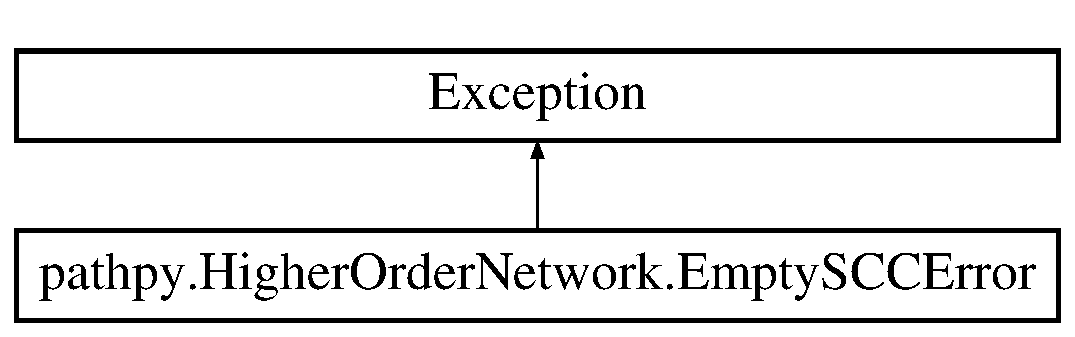
\includegraphics[height=2.000000cm]{classpathpy_1_1HigherOrderNetwork_1_1EmptySCCError}
\end{center}
\end{figure}


\subsection{Detailed Description}
\begin{DoxyVerb}This exception is thrown whenever a non-empty strongly 
connected component is needed, but we encounter an empty one
\end{DoxyVerb}
 

The documentation for this class was generated from the following file\-:\begin{DoxyCompactItemize}
\item 
/mnt/c/\-Users/ingos/\-Desktop/pathpy/pathpy/Higher\-Order\-Network.\-py\end{DoxyCompactItemize}

\hypertarget{classpathpy_1_1HigherOrderNetwork_1_1HigherOrderNetwork}{\section{pathpy.\-Higher\-Order\-Network.\-Higher\-Order\-Network Class Reference}
\label{classpathpy_1_1HigherOrderNetwork_1_1HigherOrderNetwork}\index{pathpy.\-Higher\-Order\-Network.\-Higher\-Order\-Network@{pathpy.\-Higher\-Order\-Network.\-Higher\-Order\-Network}}
}
\subsection*{Public Member Functions}
\begin{DoxyCompactItemize}
\item 
def \hyperlink{classpathpy_1_1HigherOrderNetwork_1_1HigherOrderNetwork_a63d36720423ee8d6d88c5a06f4655c84}{\-\_\-\-\_\-init\-\_\-\-\_\-}
\item 
def \hyperlink{classpathpy_1_1HigherOrderNetwork_1_1HigherOrderNetwork_a89ba7bbeb54449a87ba78eecc591fca4}{vcount}
\item 
def \hyperlink{classpathpy_1_1HigherOrderNetwork_1_1HigherOrderNetwork_ae425665357e88b0adf493854143a3f72}{ecount}
\item 
def \hyperlink{classpathpy_1_1HigherOrderNetwork_1_1HigherOrderNetwork_a91626f933af603a73f8bb39249ab6c51}{total\-Edge\-Weight}
\item 
def \hyperlink{classpathpy_1_1HigherOrderNetwork_1_1HigherOrderNetwork_a1963d0e4370e3818de3cf6886bba8594}{Higher\-Order\-Node\-To\-Path}
\item 
def \hyperlink{classpathpy_1_1HigherOrderNetwork_1_1HigherOrderNetwork_a117fe621fb02d356f6591620f9340eaa}{path\-To\-Higher\-Order\-Nodes}
\item 
def \hyperlink{classpathpy_1_1HigherOrderNetwork_1_1HigherOrderNetwork_abd69fc6003eb13d11390466182a63357}{get\-Node\-Name\-Map}
\item 
def \hyperlink{classpathpy_1_1HigherOrderNetwork_1_1HigherOrderNetwork_a3a03ec6087add6dd0b54f7264b2e21c5}{get\-Do\-F}
\item 
def \hyperlink{classpathpy_1_1HigherOrderNetwork_1_1HigherOrderNetwork_a20092d5a4a182df408af6063a0887630}{get\-Distance\-Matrix}
\item 
def \hyperlink{classpathpy_1_1HigherOrderNetwork_1_1HigherOrderNetwork_a672cdad613e84eb0f528bbc02e7c6163}{get\-Shortest\-Paths}
\item 
def \hyperlink{classpathpy_1_1HigherOrderNetwork_1_1HigherOrderNetwork_abed4839be0864210c0b5aff9376fe307}{get\-Distance\-Matrix\-First\-Order}
\item 
def \hyperlink{classpathpy_1_1HigherOrderNetwork_1_1HigherOrderNetwork_a2f94ebbc8141be6f5194ec922e3b01a0}{Closeness\-Centrality}
\item 
\hypertarget{classpathpy_1_1HigherOrderNetwork_1_1HigherOrderNetwork_a57e8494220dd4a5b2a9a45de17f9d26a}{def {\bfseries Ev\-Cent}}\label{classpathpy_1_1HigherOrderNetwork_1_1HigherOrderNetwork_a57e8494220dd4a5b2a9a45de17f9d26a}

\item 
def \hyperlink{classpathpy_1_1HigherOrderNetwork_1_1HigherOrderNetwork_abc76633f53a0747353e7ab0e15744d94}{Page\-Rank}
\item 
\hypertarget{classpathpy_1_1HigherOrderNetwork_1_1HigherOrderNetwork_ab71b78f1c9ffe7a06364841572f1fee2}{def {\bfseries Higher\-Order\-Path\-To\-First\-Order}}\label{classpathpy_1_1HigherOrderNetwork_1_1HigherOrderNetwork_ab71b78f1c9ffe7a06364841572f1fee2}

\item 
def \hyperlink{classpathpy_1_1HigherOrderNetwork_1_1HigherOrderNetwork_afcfdcfacef4f3beb7594a58600e833e4}{Betweenness\-Centrality}
\item 
def \hyperlink{classpathpy_1_1HigherOrderNetwork_1_1HigherOrderNetwork_a4b71eed8268df33814725ae7832729e6}{reduce\-To\-G\-C\-C}
\item 
def \hyperlink{classpathpy_1_1HigherOrderNetwork_1_1HigherOrderNetwork_ab35dd7f65e3bfeb280fcd38c1e7448f7}{summary}
\item 
def \hyperlink{classpathpy_1_1HigherOrderNetwork_1_1HigherOrderNetwork_a4aec883869195967a9209655905ace52}{\-\_\-\-\_\-str\-\_\-\-\_\-}
\item 
def \hyperlink{classpathpy_1_1HigherOrderNetwork_1_1HigherOrderNetwork_acd9ab003f80216ed6beff9c513a7e876}{degrees}
\item 
def \hyperlink{classpathpy_1_1HigherOrderNetwork_1_1HigherOrderNetwork_a8e10f45369dff5f7ccff3bcf7e6c5b33}{get\-Adjacency\-Matrix}
\item 
def \hyperlink{classpathpy_1_1HigherOrderNetwork_1_1HigherOrderNetwork_a20c4a62ca4706bdab81534332e3843fe}{get\-Transition\-Matrix}
\item 
def \hyperlink{classpathpy_1_1HigherOrderNetwork_1_1HigherOrderNetwork_a69ea9c565b0d8bf7f1a2d0cb409f0e15}{get\-Laplacian\-Matrix}
\item 
def \hyperlink{classpathpy_1_1HigherOrderNetwork_1_1HigherOrderNetwork_a556545310735cba27128afd37c59ed35}{get\-Eigen\-Value\-Gap}
\item 
def \hyperlink{classpathpy_1_1HigherOrderNetwork_1_1HigherOrderNetwork_a608108241f9aa06f1027d9ab84f79a65}{evcent}
\item 
def \hyperlink{classpathpy_1_1HigherOrderNetwork_1_1HigherOrderNetwork_aa8f3ed627c16c15c877fc0316c88bdb3}{get\-Fiedler\-Vector\-Sparse}
\item 
def \hyperlink{classpathpy_1_1HigherOrderNetwork_1_1HigherOrderNetwork_adea7800343373793dbd9688c77fb6191}{get\-Fiedler\-Vector\-Dense}
\item 
def \hyperlink{classpathpy_1_1HigherOrderNetwork_1_1HigherOrderNetwork_ae48d8ad635f7cf263897016d876c6fa2}{get\-Algebraic\-Connectivity}
\end{DoxyCompactItemize}
\subsection*{Static Public Member Functions}
\begin{DoxyCompactItemize}
\item 
def \hyperlink{classpathpy_1_1HigherOrderNetwork_1_1HigherOrderNetwork_a1b757112293f9093efc437ffb113df83}{get\-Leading\-Eigenvector}
\end{DoxyCompactItemize}
\subsection*{Public Attributes}
\begin{DoxyCompactItemize}
\item 
\hypertarget{classpathpy_1_1HigherOrderNetwork_1_1HigherOrderNetwork_a6dea6fe6e34178adb395ad8e79403d5c}{{\bfseries order}}\label{classpathpy_1_1HigherOrderNetwork_1_1HigherOrderNetwork_a6dea6fe6e34178adb395ad8e79403d5c}

\item 
\hypertarget{classpathpy_1_1HigherOrderNetwork_1_1HigherOrderNetwork_ac4c8ee9f7775478793d88680d6f99fc8}{{\bfseries paths}}\label{classpathpy_1_1HigherOrderNetwork_1_1HigherOrderNetwork_ac4c8ee9f7775478793d88680d6f99fc8}

\item 
\hypertarget{classpathpy_1_1HigherOrderNetwork_1_1HigherOrderNetwork_a6626777ff215fde5f7d92368a407c683}{{\bfseries nodes}}\label{classpathpy_1_1HigherOrderNetwork_1_1HigherOrderNetwork_a6626777ff215fde5f7d92368a407c683}

\item 
\hypertarget{classpathpy_1_1HigherOrderNetwork_1_1HigherOrderNetwork_af3e51491a2417e471eeb1404b44df204}{{\bfseries separator}}\label{classpathpy_1_1HigherOrderNetwork_1_1HigherOrderNetwork_af3e51491a2417e471eeb1404b44df204}

\item 
\hypertarget{classpathpy_1_1HigherOrderNetwork_1_1HigherOrderNetwork_a6eec968e72178ab2930f83928b3ca842}{{\bfseries edges}}\label{classpathpy_1_1HigherOrderNetwork_1_1HigherOrderNetwork_a6eec968e72178ab2930f83928b3ca842}

\item 
\hypertarget{classpathpy_1_1HigherOrderNetwork_1_1HigherOrderNetwork_a522350b2e4a401732b64bb0acf1634ea}{{\bfseries successors}}\label{classpathpy_1_1HigherOrderNetwork_1_1HigherOrderNetwork_a522350b2e4a401732b64bb0acf1634ea}

\item 
\hypertarget{classpathpy_1_1HigherOrderNetwork_1_1HigherOrderNetwork_a8a271893d9fb656f805e36335afca257}{{\bfseries dof\-\_\-paths}}\label{classpathpy_1_1HigherOrderNetwork_1_1HigherOrderNetwork_a8a271893d9fb656f805e36335afca257}

\item 
\hypertarget{classpathpy_1_1HigherOrderNetwork_1_1HigherOrderNetwork_a25d69b9cc9b7b328fbd201244e68ca95}{{\bfseries dof\-\_\-ngrams}}\label{classpathpy_1_1HigherOrderNetwork_1_1HigherOrderNetwork_a25d69b9cc9b7b328fbd201244e68ca95}

\end{DoxyCompactItemize}


\subsection{Detailed Description}
\begin{DoxyVerb}Instances of this class capture a k-th-order representation of path statistics. Path statistics 
can originate from pathway data, temporal networks, or from processes observed on top of a network topology.
\end{DoxyVerb}
 

\subsection{Constructor \& Destructor Documentation}
\hypertarget{classpathpy_1_1HigherOrderNetwork_1_1HigherOrderNetwork_a63d36720423ee8d6d88c5a06f4655c84}{\index{pathpy\-::\-Higher\-Order\-Network\-::\-Higher\-Order\-Network@{pathpy\-::\-Higher\-Order\-Network\-::\-Higher\-Order\-Network}!\-\_\-\-\_\-init\-\_\-\-\_\-@{\-\_\-\-\_\-init\-\_\-\-\_\-}}
\index{\-\_\-\-\_\-init\-\_\-\-\_\-@{\-\_\-\-\_\-init\-\_\-\-\_\-}!pathpy::HigherOrderNetwork::HigherOrderNetwork@{pathpy\-::\-Higher\-Order\-Network\-::\-Higher\-Order\-Network}}
\subsubsection[{\-\_\-\-\_\-init\-\_\-\-\_\-}]{\setlength{\rightskip}{0pt plus 5cm}def pathpy.\-Higher\-Order\-Network.\-Higher\-Order\-Network.\-\_\-\-\_\-init\-\_\-\-\_\- (
\begin{DoxyParamCaption}
\item[{}]{self, }
\item[{}]{paths, }
\item[{}]{k = {\ttfamily 1}, }
\item[{}]{separator = {\ttfamily '-\/'}, }
\item[{}]{null\-Model = {\ttfamily False}, }
\item[{}]{method = {\ttfamily 'FirstOrderTransitions'}, }
\item[{}]{lanczos\-Vecs = {\ttfamily 15}, }
\item[{}]{maxiter = {\ttfamily 1000}}
\end{DoxyParamCaption}
)}}\label{classpathpy_1_1HigherOrderNetwork_1_1HigherOrderNetwork_a63d36720423ee8d6d88c5a06f4655c84}
\begin{DoxyVerb}Generates a k-th-order representation based on the given path statistics.

@param paths: An instance of class Paths, which contains the path statistics to be 
    used in the generation of the k-th order representation 

@param k: The order of the network representation to generate. For the default case of 
    k=1, the resulting representation corresponds to the usual (first-order) aggregate network, 
    i.e. links connect nodes and link weights are given by the frequency of each interaction. For 
    k>1, a k-th order node corresponds to a sequence of k nodes. The weight of a k-th order link 
    captures the frequency of a path of length k.

@param separator: The separator character to be used in higher-order node names.

@param nullModel: For the default value False, link weights are generated based on the statistics of 
    paths of length k in the underlying path statistics instance. If True, link weights are generated 
    from the first-order model (k=1) based on the assumption of independent links (i.e. corresponding) 
    to a first-order Markov model.

@param method: specifies how the null model link weights in the k-th order model are calculated. 
    For the default method='FirstOrderTransitions', the weight w('v_1-v_2-...v_k', 'v_2-...-v_k-v_k+1') of 
    a k-order edge is set to the transition probability T['v_k', 'v_k+1'] in the first order network.
    For method='KOrderPi' the entry pi['v1-...-v_k'] in the stationary distribution of the 
    k-order network is used instead.
\end{DoxyVerb}
 

\subsection{Member Function Documentation}
\hypertarget{classpathpy_1_1HigherOrderNetwork_1_1HigherOrderNetwork_a4aec883869195967a9209655905ace52}{\index{pathpy\-::\-Higher\-Order\-Network\-::\-Higher\-Order\-Network@{pathpy\-::\-Higher\-Order\-Network\-::\-Higher\-Order\-Network}!\-\_\-\-\_\-str\-\_\-\-\_\-@{\-\_\-\-\_\-str\-\_\-\-\_\-}}
\index{\-\_\-\-\_\-str\-\_\-\-\_\-@{\-\_\-\-\_\-str\-\_\-\-\_\-}!pathpy::HigherOrderNetwork::HigherOrderNetwork@{pathpy\-::\-Higher\-Order\-Network\-::\-Higher\-Order\-Network}}
\subsubsection[{\-\_\-\-\_\-str\-\_\-\-\_\-}]{\setlength{\rightskip}{0pt plus 5cm}def pathpy.\-Higher\-Order\-Network.\-Higher\-Order\-Network.\-\_\-\-\_\-str\-\_\-\-\_\- (
\begin{DoxyParamCaption}
\item[{}]{self}
\end{DoxyParamCaption}
)}}\label{classpathpy_1_1HigherOrderNetwork_1_1HigherOrderNetwork_a4aec883869195967a9209655905ace52}
\begin{DoxyVerb}Returns the default string representation of 
this graphical model instance
\end{DoxyVerb}
 \hypertarget{classpathpy_1_1HigherOrderNetwork_1_1HigherOrderNetwork_afcfdcfacef4f3beb7594a58600e833e4}{\index{pathpy\-::\-Higher\-Order\-Network\-::\-Higher\-Order\-Network@{pathpy\-::\-Higher\-Order\-Network\-::\-Higher\-Order\-Network}!Betweenness\-Centrality@{Betweenness\-Centrality}}
\index{Betweenness\-Centrality@{Betweenness\-Centrality}!pathpy::HigherOrderNetwork::HigherOrderNetwork@{pathpy\-::\-Higher\-Order\-Network\-::\-Higher\-Order\-Network}}
\subsubsection[{Betweenness\-Centrality}]{\setlength{\rightskip}{0pt plus 5cm}def pathpy.\-Higher\-Order\-Network.\-Higher\-Order\-Network.\-Betweenness\-Centrality (
\begin{DoxyParamCaption}
\item[{}]{self, }
\item[{}]{normalized = {\ttfamily False}}
\end{DoxyParamCaption}
)}}\label{classpathpy_1_1HigherOrderNetwork_1_1HigherOrderNetwork_afcfdcfacef4f3beb7594a58600e833e4}
\begin{DoxyVerb}Calculates the betweenness centralities of all nodes.
If the order of the higher-order network is larger than one 
centralities calculated based on the higher-order 
topology will automatically be projected back to first-order 
nodes.
\end{DoxyVerb}
 \hypertarget{classpathpy_1_1HigherOrderNetwork_1_1HigherOrderNetwork_a2f94ebbc8141be6f5194ec922e3b01a0}{\index{pathpy\-::\-Higher\-Order\-Network\-::\-Higher\-Order\-Network@{pathpy\-::\-Higher\-Order\-Network\-::\-Higher\-Order\-Network}!Closeness\-Centrality@{Closeness\-Centrality}}
\index{Closeness\-Centrality@{Closeness\-Centrality}!pathpy::HigherOrderNetwork::HigherOrderNetwork@{pathpy\-::\-Higher\-Order\-Network\-::\-Higher\-Order\-Network}}
\subsubsection[{Closeness\-Centrality}]{\setlength{\rightskip}{0pt plus 5cm}def pathpy.\-Higher\-Order\-Network.\-Higher\-Order\-Network.\-Closeness\-Centrality (
\begin{DoxyParamCaption}
\item[{}]{self}
\end{DoxyParamCaption}
)}}\label{classpathpy_1_1HigherOrderNetwork_1_1HigherOrderNetwork_a2f94ebbc8141be6f5194ec922e3b01a0}
\begin{DoxyVerb}Calculates the closeness centralities of all nodes.
If the order of the higher-order network is larger than one 
centralities calculated based on the higher-order 
topology will automatically be projected back to first-order 
nodes.
\end{DoxyVerb}
 \hypertarget{classpathpy_1_1HigherOrderNetwork_1_1HigherOrderNetwork_acd9ab003f80216ed6beff9c513a7e876}{\index{pathpy\-::\-Higher\-Order\-Network\-::\-Higher\-Order\-Network@{pathpy\-::\-Higher\-Order\-Network\-::\-Higher\-Order\-Network}!degrees@{degrees}}
\index{degrees@{degrees}!pathpy::HigherOrderNetwork::HigherOrderNetwork@{pathpy\-::\-Higher\-Order\-Network\-::\-Higher\-Order\-Network}}
\subsubsection[{degrees}]{\setlength{\rightskip}{0pt plus 5cm}def pathpy.\-Higher\-Order\-Network.\-Higher\-Order\-Network.\-degrees (
\begin{DoxyParamCaption}
\item[{}]{self, }
\item[{}]{include\-Sub\-Paths = {\ttfamily True}, }
\item[{}]{weighted = {\ttfamily True}, }
\item[{}]{mode = {\ttfamily \char`\"{}OUT\char`\"{}}}
\end{DoxyParamCaption}
)}}\label{classpathpy_1_1HigherOrderNetwork_1_1HigherOrderNetwork_acd9ab003f80216ed6beff9c513a7e876}
\begin{DoxyVerb}Returns the (weighted) degrees of nodes in the higher-order network

@param weighted: If true, calculates the sum of weights for each node. If false, the 
    number of links is calculated

@param mode: either "IN", "OUT", or "TOTAL" 
\end{DoxyVerb}
 \hypertarget{classpathpy_1_1HigherOrderNetwork_1_1HigherOrderNetwork_ae425665357e88b0adf493854143a3f72}{\index{pathpy\-::\-Higher\-Order\-Network\-::\-Higher\-Order\-Network@{pathpy\-::\-Higher\-Order\-Network\-::\-Higher\-Order\-Network}!ecount@{ecount}}
\index{ecount@{ecount}!pathpy::HigherOrderNetwork::HigherOrderNetwork@{pathpy\-::\-Higher\-Order\-Network\-::\-Higher\-Order\-Network}}
\subsubsection[{ecount}]{\setlength{\rightskip}{0pt plus 5cm}def pathpy.\-Higher\-Order\-Network.\-Higher\-Order\-Network.\-ecount (
\begin{DoxyParamCaption}
\item[{}]{self}
\end{DoxyParamCaption}
)}}\label{classpathpy_1_1HigherOrderNetwork_1_1HigherOrderNetwork_ae425665357e88b0adf493854143a3f72}
\begin{DoxyVerb}Returns the number of links \end{DoxyVerb}
 \hypertarget{classpathpy_1_1HigherOrderNetwork_1_1HigherOrderNetwork_a608108241f9aa06f1027d9ab84f79a65}{\index{pathpy\-::\-Higher\-Order\-Network\-::\-Higher\-Order\-Network@{pathpy\-::\-Higher\-Order\-Network\-::\-Higher\-Order\-Network}!evcent@{evcent}}
\index{evcent@{evcent}!pathpy::HigherOrderNetwork::HigherOrderNetwork@{pathpy\-::\-Higher\-Order\-Network\-::\-Higher\-Order\-Network}}
\subsubsection[{evcent}]{\setlength{\rightskip}{0pt plus 5cm}def pathpy.\-Higher\-Order\-Network.\-Higher\-Order\-Network.\-evcent (
\begin{DoxyParamCaption}
\item[{}]{self, }
\item[{}]{normalized = {\ttfamily True}}
\end{DoxyParamCaption}
)}}\label{classpathpy_1_1HigherOrderNetwork_1_1HigherOrderNetwork_a608108241f9aa06f1027d9ab84f79a65}
\begin{DoxyVerb}Computes eigenvector centralities of nodes in the higher-order network. 
If order>1, centralities are aggregated to obtain the eigenvector centrality 
of first-order nodes (but based on the higher-order model).
\end{DoxyVerb}
 \hypertarget{classpathpy_1_1HigherOrderNetwork_1_1HigherOrderNetwork_a8e10f45369dff5f7ccff3bcf7e6c5b33}{\index{pathpy\-::\-Higher\-Order\-Network\-::\-Higher\-Order\-Network@{pathpy\-::\-Higher\-Order\-Network\-::\-Higher\-Order\-Network}!get\-Adjacency\-Matrix@{get\-Adjacency\-Matrix}}
\index{get\-Adjacency\-Matrix@{get\-Adjacency\-Matrix}!pathpy::HigherOrderNetwork::HigherOrderNetwork@{pathpy\-::\-Higher\-Order\-Network\-::\-Higher\-Order\-Network}}
\subsubsection[{get\-Adjacency\-Matrix}]{\setlength{\rightskip}{0pt plus 5cm}def pathpy.\-Higher\-Order\-Network.\-Higher\-Order\-Network.\-get\-Adjacency\-Matrix (
\begin{DoxyParamCaption}
\item[{}]{self, }
\item[{}]{include\-Sub\-Paths = {\ttfamily True}, }
\item[{}]{weighted = {\ttfamily True}, }
\item[{}]{transposed = {\ttfamily False}}
\end{DoxyParamCaption}
)}}\label{classpathpy_1_1HigherOrderNetwork_1_1HigherOrderNetwork_a8e10f45369dff5f7ccff3bcf7e6c5b33}
\begin{DoxyVerb}Returns a sparse adjacency matrix of the higher-order network. By default, the entry 
    corresponding to a directed link source -> target is stored in row s and column t
    and can be accessed via A[s,t].
    
@param includeSubPaths: if set to True, the returned adjacency matrix will 
    account for the occurrence of links of order k (i.e. paths of length k-1)
    as subpaths

@param weighted: if set to False, the function returns a binary adjacency matrix.
  If set to True, adjacency matrix entries will contain the weight of an edge.
      
@param transposed: whether to transpose the matrix or not.
\end{DoxyVerb}
 \hypertarget{classpathpy_1_1HigherOrderNetwork_1_1HigherOrderNetwork_ae48d8ad635f7cf263897016d876c6fa2}{\index{pathpy\-::\-Higher\-Order\-Network\-::\-Higher\-Order\-Network@{pathpy\-::\-Higher\-Order\-Network\-::\-Higher\-Order\-Network}!get\-Algebraic\-Connectivity@{get\-Algebraic\-Connectivity}}
\index{get\-Algebraic\-Connectivity@{get\-Algebraic\-Connectivity}!pathpy::HigherOrderNetwork::HigherOrderNetwork@{pathpy\-::\-Higher\-Order\-Network\-::\-Higher\-Order\-Network}}
\subsubsection[{get\-Algebraic\-Connectivity}]{\setlength{\rightskip}{0pt plus 5cm}def pathpy.\-Higher\-Order\-Network.\-Higher\-Order\-Network.\-get\-Algebraic\-Connectivity (
\begin{DoxyParamCaption}
\item[{}]{self, }
\item[{}]{lanczos\-Vecs = {\ttfamily 15}, }
\item[{}]{maxiter = {\ttfamily 20}}
\end{DoxyParamCaption}
)}}\label{classpathpy_1_1HigherOrderNetwork_1_1HigherOrderNetwork_ae48d8ad635f7cf263897016d876c6fa2}
\begin{DoxyVerb}Returns the algebraic connectivity of the higher-order network.    

@param lanczosVecs: number of Lanczos vectors to be used in the approximate
    calculation of eigenvectors and eigenvalues. This maps to the ncv parameter 
    of scipy's underlying function eigs. 
@param maxiter: scaling factor for the number of iterations to be used in the 
    approximate calculation of eigenvectors and eigenvalues. The number of iterations 
    passed to scipy's underlying eigs function will be n*maxiter where n is the
    number of rows/columns of the Laplacian matrix.         
\end{DoxyVerb}
 \hypertarget{classpathpy_1_1HigherOrderNetwork_1_1HigherOrderNetwork_a20092d5a4a182df408af6063a0887630}{\index{pathpy\-::\-Higher\-Order\-Network\-::\-Higher\-Order\-Network@{pathpy\-::\-Higher\-Order\-Network\-::\-Higher\-Order\-Network}!get\-Distance\-Matrix@{get\-Distance\-Matrix}}
\index{get\-Distance\-Matrix@{get\-Distance\-Matrix}!pathpy::HigherOrderNetwork::HigherOrderNetwork@{pathpy\-::\-Higher\-Order\-Network\-::\-Higher\-Order\-Network}}
\subsubsection[{get\-Distance\-Matrix}]{\setlength{\rightskip}{0pt plus 5cm}def pathpy.\-Higher\-Order\-Network.\-Higher\-Order\-Network.\-get\-Distance\-Matrix (
\begin{DoxyParamCaption}
\item[{}]{self}
\end{DoxyParamCaption}
)}}\label{classpathpy_1_1HigherOrderNetwork_1_1HigherOrderNetwork_a20092d5a4a182df408af6063a0887630}
\begin{DoxyVerb}Calculates shortest path distances between all pairs of 
higher-order nodes using the Floyd-Warshall algorithm.
\end{DoxyVerb}
 \hypertarget{classpathpy_1_1HigherOrderNetwork_1_1HigherOrderNetwork_abed4839be0864210c0b5aff9376fe307}{\index{pathpy\-::\-Higher\-Order\-Network\-::\-Higher\-Order\-Network@{pathpy\-::\-Higher\-Order\-Network\-::\-Higher\-Order\-Network}!get\-Distance\-Matrix\-First\-Order@{get\-Distance\-Matrix\-First\-Order}}
\index{get\-Distance\-Matrix\-First\-Order@{get\-Distance\-Matrix\-First\-Order}!pathpy::HigherOrderNetwork::HigherOrderNetwork@{pathpy\-::\-Higher\-Order\-Network\-::\-Higher\-Order\-Network}}
\subsubsection[{get\-Distance\-Matrix\-First\-Order}]{\setlength{\rightskip}{0pt plus 5cm}def pathpy.\-Higher\-Order\-Network.\-Higher\-Order\-Network.\-get\-Distance\-Matrix\-First\-Order (
\begin{DoxyParamCaption}
\item[{}]{self}
\end{DoxyParamCaption}
)}}\label{classpathpy_1_1HigherOrderNetwork_1_1HigherOrderNetwork_abed4839be0864210c0b5aff9376fe307}
\begin{DoxyVerb}Projects a distance matrix from a higher-order to 
first-order nodes, while path lengths are calculated 
based on the higher-order topology
\end{DoxyVerb}
 \hypertarget{classpathpy_1_1HigherOrderNetwork_1_1HigherOrderNetwork_a3a03ec6087add6dd0b54f7264b2e21c5}{\index{pathpy\-::\-Higher\-Order\-Network\-::\-Higher\-Order\-Network@{pathpy\-::\-Higher\-Order\-Network\-::\-Higher\-Order\-Network}!get\-Do\-F@{get\-Do\-F}}
\index{get\-Do\-F@{get\-Do\-F}!pathpy::HigherOrderNetwork::HigherOrderNetwork@{pathpy\-::\-Higher\-Order\-Network\-::\-Higher\-Order\-Network}}
\subsubsection[{get\-Do\-F}]{\setlength{\rightskip}{0pt plus 5cm}def pathpy.\-Higher\-Order\-Network.\-Higher\-Order\-Network.\-get\-Do\-F (
\begin{DoxyParamCaption}
\item[{}]{self, }
\item[{}]{assumption = {\ttfamily \char`\"{}paths\char`\"{}}}
\end{DoxyParamCaption}
)}}\label{classpathpy_1_1HigherOrderNetwork_1_1HigherOrderNetwork_a3a03ec6087add6dd0b54f7264b2e21c5}
\begin{DoxyVerb}Calculates the degrees of freedom (i.e. number of parameters) of 
this k-order model. Depending on the modeling assumptions, this either
corresponds to the number of paths of length k in the first-order network 
or to the number of all possible k-grams. The degrees of freedom of a model 
can be used to assess the model complexity when calculating, e.g., the 
Bayesian Information Criterion (BIC).

@param assumption: if set to 'paths', for the degree of freedon calculation in the BIC, 
    only paths in the first-order network topology will be considered. This is 
    needed whenever we are interested in a modeling of paths in a given network topology.
    If set to 'ngrams' all possible n-grams will be considered, independent of whether they 
    are valid paths in the first-order network or not. The 'ngrams' and the 'paths' assumption 
    coincide if the first-order network is fully connected.
\end{DoxyVerb}
 \hypertarget{classpathpy_1_1HigherOrderNetwork_1_1HigherOrderNetwork_a556545310735cba27128afd37c59ed35}{\index{pathpy\-::\-Higher\-Order\-Network\-::\-Higher\-Order\-Network@{pathpy\-::\-Higher\-Order\-Network\-::\-Higher\-Order\-Network}!get\-Eigen\-Value\-Gap@{get\-Eigen\-Value\-Gap}}
\index{get\-Eigen\-Value\-Gap@{get\-Eigen\-Value\-Gap}!pathpy::HigherOrderNetwork::HigherOrderNetwork@{pathpy\-::\-Higher\-Order\-Network\-::\-Higher\-Order\-Network}}
\subsubsection[{get\-Eigen\-Value\-Gap}]{\setlength{\rightskip}{0pt plus 5cm}def pathpy.\-Higher\-Order\-Network.\-Higher\-Order\-Network.\-get\-Eigen\-Value\-Gap (
\begin{DoxyParamCaption}
\item[{}]{self, }
\item[{}]{include\-Sub\-Paths = {\ttfamily True}, }
\item[{}]{lanczos\-Vecs = {\ttfamily 15}, }
\item[{}]{maxiter = {\ttfamily 20}}
\end{DoxyParamCaption}
)}}\label{classpathpy_1_1HigherOrderNetwork_1_1HigherOrderNetwork_a556545310735cba27128afd37c59ed35}
\begin{DoxyVerb}Returns the eigenvalue gap of the transition matrix    
\end{DoxyVerb}
 \hypertarget{classpathpy_1_1HigherOrderNetwork_1_1HigherOrderNetwork_adea7800343373793dbd9688c77fb6191}{\index{pathpy\-::\-Higher\-Order\-Network\-::\-Higher\-Order\-Network@{pathpy\-::\-Higher\-Order\-Network\-::\-Higher\-Order\-Network}!get\-Fiedler\-Vector\-Dense@{get\-Fiedler\-Vector\-Dense}}
\index{get\-Fiedler\-Vector\-Dense@{get\-Fiedler\-Vector\-Dense}!pathpy::HigherOrderNetwork::HigherOrderNetwork@{pathpy\-::\-Higher\-Order\-Network\-::\-Higher\-Order\-Network}}
\subsubsection[{get\-Fiedler\-Vector\-Dense}]{\setlength{\rightskip}{0pt plus 5cm}def pathpy.\-Higher\-Order\-Network.\-Higher\-Order\-Network.\-get\-Fiedler\-Vector\-Dense (
\begin{DoxyParamCaption}
\item[{}]{self}
\end{DoxyParamCaption}
)}}\label{classpathpy_1_1HigherOrderNetwork_1_1HigherOrderNetwork_adea7800343373793dbd9688c77fb6191}
\begin{DoxyVerb} Returns the (dense)Fiedler vector of the higher-order network. The Fiedler 
 vector can be used for a spectral bisectioning of the network.             
\end{DoxyVerb}
 \hypertarget{classpathpy_1_1HigherOrderNetwork_1_1HigherOrderNetwork_aa8f3ed627c16c15c877fc0316c88bdb3}{\index{pathpy\-::\-Higher\-Order\-Network\-::\-Higher\-Order\-Network@{pathpy\-::\-Higher\-Order\-Network\-::\-Higher\-Order\-Network}!get\-Fiedler\-Vector\-Sparse@{get\-Fiedler\-Vector\-Sparse}}
\index{get\-Fiedler\-Vector\-Sparse@{get\-Fiedler\-Vector\-Sparse}!pathpy::HigherOrderNetwork::HigherOrderNetwork@{pathpy\-::\-Higher\-Order\-Network\-::\-Higher\-Order\-Network}}
\subsubsection[{get\-Fiedler\-Vector\-Sparse}]{\setlength{\rightskip}{0pt plus 5cm}def pathpy.\-Higher\-Order\-Network.\-Higher\-Order\-Network.\-get\-Fiedler\-Vector\-Sparse (
\begin{DoxyParamCaption}
\item[{}]{self, }
\item[{}]{normalized = {\ttfamily True}, }
\item[{}]{lanczos\-Vecs = {\ttfamily 15}, }
\item[{}]{maxiter = {\ttfamily 20}}
\end{DoxyParamCaption}
)}}\label{classpathpy_1_1HigherOrderNetwork_1_1HigherOrderNetwork_aa8f3ed627c16c15c877fc0316c88bdb3}
\begin{DoxyVerb}Returns the (sparse) Fiedler vector of the higher-order network. The Fiedler 
vector can be used for a spectral bisectioning of the network.
     
Note that sparse linear algebra for eigenvalue problems with small eigenvalues 
is problematic in terms of numerical stability. Consider using the dense version
of this method in this case. Note also that the sparse Fiedler vector might be scaled by 
a factor (-1) compared to the dense version.
  
@param normalized: whether (default) or not to normalize the fiedler vector.
  Normalization is done such that the sum of squares equals one in order to
  get reasonable values as entries might be positive and negative.
@param lanczosVecs: number of Lanczos vectors to be used in the approximate
    calculation of eigenvectors and eigenvalues. This maps to the ncv parameter 
    of scipy's underlying function eigs. 
@param maxiter: scaling factor for the number of iterations to be used in the 
    approximate calculation of eigenvectors and eigenvalues. The number of iterations 
    passed to scipy's underlying eigs function will be n*maxiter where n is the 
    number of rows/columns of the Laplacian matrix.
\end{DoxyVerb}
 \hypertarget{classpathpy_1_1HigherOrderNetwork_1_1HigherOrderNetwork_a69ea9c565b0d8bf7f1a2d0cb409f0e15}{\index{pathpy\-::\-Higher\-Order\-Network\-::\-Higher\-Order\-Network@{pathpy\-::\-Higher\-Order\-Network\-::\-Higher\-Order\-Network}!get\-Laplacian\-Matrix@{get\-Laplacian\-Matrix}}
\index{get\-Laplacian\-Matrix@{get\-Laplacian\-Matrix}!pathpy::HigherOrderNetwork::HigherOrderNetwork@{pathpy\-::\-Higher\-Order\-Network\-::\-Higher\-Order\-Network}}
\subsubsection[{get\-Laplacian\-Matrix}]{\setlength{\rightskip}{0pt plus 5cm}def pathpy.\-Higher\-Order\-Network.\-Higher\-Order\-Network.\-get\-Laplacian\-Matrix (
\begin{DoxyParamCaption}
\item[{}]{self, }
\item[{}]{include\-Sub\-Paths = {\ttfamily True}}
\end{DoxyParamCaption}
)}}\label{classpathpy_1_1HigherOrderNetwork_1_1HigherOrderNetwork_a69ea9c565b0d8bf7f1a2d0cb409f0e15}
\begin{DoxyVerb}Returns the transposed Laplacian matrix corresponding to the higher-order network.                
\end{DoxyVerb}
 \hypertarget{classpathpy_1_1HigherOrderNetwork_1_1HigherOrderNetwork_a1b757112293f9093efc437ffb113df83}{\index{pathpy\-::\-Higher\-Order\-Network\-::\-Higher\-Order\-Network@{pathpy\-::\-Higher\-Order\-Network\-::\-Higher\-Order\-Network}!get\-Leading\-Eigenvector@{get\-Leading\-Eigenvector}}
\index{get\-Leading\-Eigenvector@{get\-Leading\-Eigenvector}!pathpy::HigherOrderNetwork::HigherOrderNetwork@{pathpy\-::\-Higher\-Order\-Network\-::\-Higher\-Order\-Network}}
\subsubsection[{get\-Leading\-Eigenvector}]{\setlength{\rightskip}{0pt plus 5cm}def pathpy.\-Higher\-Order\-Network.\-Higher\-Order\-Network.\-get\-Leading\-Eigenvector (
\begin{DoxyParamCaption}
\item[{}]{A, }
\item[{}]{normalized = {\ttfamily True}, }
\item[{}]{lanczos\-Vecs = {\ttfamily 15}, }
\item[{}]{maxiter = {\ttfamily 1000}}
\end{DoxyParamCaption}
)\hspace{0.3cm}{\ttfamily [static]}}}\label{classpathpy_1_1HigherOrderNetwork_1_1HigherOrderNetwork_a1b757112293f9093efc437ffb113df83}
\begin{DoxyVerb}Compute normalized leading eigenvector of a given matrix A.

@param A: sparse matrix for which leading eigenvector will be computed
@param normalized: wheter or not to normalize. Default is C{True}
@param lanczosVecs: number of Lanczos vectors to be used in the approximate
    calculation of eigenvectors and eigenvalues. This maps to the ncv parameter 
    of scipy's underlying function eigs. 
@param maxiter: scaling factor for the number of iterations to be used in the 
    approximate calculation of eigenvectors and eigenvalues. The number of iterations 
    passed to scipy's underlying eigs function will be n*maxiter where n is the 
    number of rows/columns of the Laplacian matrix.
\end{DoxyVerb}
 \hypertarget{classpathpy_1_1HigherOrderNetwork_1_1HigherOrderNetwork_abd69fc6003eb13d11390466182a63357}{\index{pathpy\-::\-Higher\-Order\-Network\-::\-Higher\-Order\-Network@{pathpy\-::\-Higher\-Order\-Network\-::\-Higher\-Order\-Network}!get\-Node\-Name\-Map@{get\-Node\-Name\-Map}}
\index{get\-Node\-Name\-Map@{get\-Node\-Name\-Map}!pathpy::HigherOrderNetwork::HigherOrderNetwork@{pathpy\-::\-Higher\-Order\-Network\-::\-Higher\-Order\-Network}}
\subsubsection[{get\-Node\-Name\-Map}]{\setlength{\rightskip}{0pt plus 5cm}def pathpy.\-Higher\-Order\-Network.\-Higher\-Order\-Network.\-get\-Node\-Name\-Map (
\begin{DoxyParamCaption}
\item[{}]{self}
\end{DoxyParamCaption}
)}}\label{classpathpy_1_1HigherOrderNetwork_1_1HigherOrderNetwork_abd69fc6003eb13d11390466182a63357}
\begin{DoxyVerb}Returns a dictionary that can be used to map 
node nodes to matrix/vector indices
\end{DoxyVerb}
 \hypertarget{classpathpy_1_1HigherOrderNetwork_1_1HigherOrderNetwork_a672cdad613e84eb0f528bbc02e7c6163}{\index{pathpy\-::\-Higher\-Order\-Network\-::\-Higher\-Order\-Network@{pathpy\-::\-Higher\-Order\-Network\-::\-Higher\-Order\-Network}!get\-Shortest\-Paths@{get\-Shortest\-Paths}}
\index{get\-Shortest\-Paths@{get\-Shortest\-Paths}!pathpy::HigherOrderNetwork::HigherOrderNetwork@{pathpy\-::\-Higher\-Order\-Network\-::\-Higher\-Order\-Network}}
\subsubsection[{get\-Shortest\-Paths}]{\setlength{\rightskip}{0pt plus 5cm}def pathpy.\-Higher\-Order\-Network.\-Higher\-Order\-Network.\-get\-Shortest\-Paths (
\begin{DoxyParamCaption}
\item[{}]{self}
\end{DoxyParamCaption}
)}}\label{classpathpy_1_1HigherOrderNetwork_1_1HigherOrderNetwork_a672cdad613e84eb0f528bbc02e7c6163}
\begin{DoxyVerb}Calculates all shortest paths between all pairs of 
higher-order nodes using the Floyd-Warshall algorithm.
\end{DoxyVerb}
 \hypertarget{classpathpy_1_1HigherOrderNetwork_1_1HigherOrderNetwork_a20c4a62ca4706bdab81534332e3843fe}{\index{pathpy\-::\-Higher\-Order\-Network\-::\-Higher\-Order\-Network@{pathpy\-::\-Higher\-Order\-Network\-::\-Higher\-Order\-Network}!get\-Transition\-Matrix@{get\-Transition\-Matrix}}
\index{get\-Transition\-Matrix@{get\-Transition\-Matrix}!pathpy::HigherOrderNetwork::HigherOrderNetwork@{pathpy\-::\-Higher\-Order\-Network\-::\-Higher\-Order\-Network}}
\subsubsection[{get\-Transition\-Matrix}]{\setlength{\rightskip}{0pt plus 5cm}def pathpy.\-Higher\-Order\-Network.\-Higher\-Order\-Network.\-get\-Transition\-Matrix (
\begin{DoxyParamCaption}
\item[{}]{self, }
\item[{}]{include\-Sub\-Paths = {\ttfamily True}}
\end{DoxyParamCaption}
)}}\label{classpathpy_1_1HigherOrderNetwork_1_1HigherOrderNetwork_a20c4a62ca4706bdab81534332e3843fe}
\begin{DoxyVerb}Returns a (transposed) random walk transition matrix 
corresponding to the higher-order network    
\end{DoxyVerb}
 \hypertarget{classpathpy_1_1HigherOrderNetwork_1_1HigherOrderNetwork_a1963d0e4370e3818de3cf6886bba8594}{\index{pathpy\-::\-Higher\-Order\-Network\-::\-Higher\-Order\-Network@{pathpy\-::\-Higher\-Order\-Network\-::\-Higher\-Order\-Network}!Higher\-Order\-Node\-To\-Path@{Higher\-Order\-Node\-To\-Path}}
\index{Higher\-Order\-Node\-To\-Path@{Higher\-Order\-Node\-To\-Path}!pathpy::HigherOrderNetwork::HigherOrderNetwork@{pathpy\-::\-Higher\-Order\-Network\-::\-Higher\-Order\-Network}}
\subsubsection[{Higher\-Order\-Node\-To\-Path}]{\setlength{\rightskip}{0pt plus 5cm}def pathpy.\-Higher\-Order\-Network.\-Higher\-Order\-Network.\-Higher\-Order\-Node\-To\-Path (
\begin{DoxyParamCaption}
\item[{}]{self, }
\item[{}]{node}
\end{DoxyParamCaption}
)}}\label{classpathpy_1_1HigherOrderNetwork_1_1HigherOrderNetwork_a1963d0e4370e3818de3cf6886bba8594}
\begin{DoxyVerb}Helper function that transforms a node in a
higher-order network of order k into a corresponding 
path of length k-1
\end{DoxyVerb}
 \hypertarget{classpathpy_1_1HigherOrderNetwork_1_1HigherOrderNetwork_abc76633f53a0747353e7ab0e15744d94}{\index{pathpy\-::\-Higher\-Order\-Network\-::\-Higher\-Order\-Network@{pathpy\-::\-Higher\-Order\-Network\-::\-Higher\-Order\-Network}!Page\-Rank@{Page\-Rank}}
\index{Page\-Rank@{Page\-Rank}!pathpy::HigherOrderNetwork::HigherOrderNetwork@{pathpy\-::\-Higher\-Order\-Network\-::\-Higher\-Order\-Network}}
\subsubsection[{Page\-Rank}]{\setlength{\rightskip}{0pt plus 5cm}def pathpy.\-Higher\-Order\-Network.\-Higher\-Order\-Network.\-Page\-Rank (
\begin{DoxyParamCaption}
\item[{}]{self, }
\item[{}]{alpha = {\ttfamily 0.85}, }
\item[{}]{max\-Iterations = {\ttfamily 100}, }
\item[{}]{convergence\-Thres = {\ttfamily 1.0e-\/6}, }
\item[{}]{projection = {\ttfamily 'scaled'}, }
\item[{}]{include\-Sub\-Paths = {\ttfamily True}}
\end{DoxyParamCaption}
)}}\label{classpathpy_1_1HigherOrderNetwork_1_1HigherOrderNetwork_abc76633f53a0747353e7ab0e15744d94}
\begin{DoxyVerb}Calculates the PageRank of higher-order nodes based on a 
power iteration. If the order of the higher-order network is larger than one,
the PageRank calculated based on the higher-order
topology will automatically be projected back to first-order 
nodes.

@param projection: Indicates how the projection from k-th-order nodes (v1, v2, ... , v{k-1})
    shall be performed. For the default method 'all', the pagerank value of the higher-order node 
    will be added to *all* first-order nodes on the path corresponding to the higher-order node. For 
    the method 'last', the PR value of the higher-order node will only be assigned to *last* 
    first-order node v{k-1}.
\end{DoxyVerb}
 \hypertarget{classpathpy_1_1HigherOrderNetwork_1_1HigherOrderNetwork_a117fe621fb02d356f6591620f9340eaa}{\index{pathpy\-::\-Higher\-Order\-Network\-::\-Higher\-Order\-Network@{pathpy\-::\-Higher\-Order\-Network\-::\-Higher\-Order\-Network}!path\-To\-Higher\-Order\-Nodes@{path\-To\-Higher\-Order\-Nodes}}
\index{path\-To\-Higher\-Order\-Nodes@{path\-To\-Higher\-Order\-Nodes}!pathpy::HigherOrderNetwork::HigherOrderNetwork@{pathpy\-::\-Higher\-Order\-Network\-::\-Higher\-Order\-Network}}
\subsubsection[{path\-To\-Higher\-Order\-Nodes}]{\setlength{\rightskip}{0pt plus 5cm}def pathpy.\-Higher\-Order\-Network.\-Higher\-Order\-Network.\-path\-To\-Higher\-Order\-Nodes (
\begin{DoxyParamCaption}
\item[{}]{self, }
\item[{}]{path, }
\item[{}]{k = {\ttfamily None}}
\end{DoxyParamCaption}
)}}\label{classpathpy_1_1HigherOrderNetwork_1_1HigherOrderNetwork_a117fe621fb02d356f6591620f9340eaa}
\begin{DoxyVerb}Helper function that transforms a path into a sequence of k-order nodes 
using the separator character of the HigherOrderNetwork instance 

Consider an example path (a,b,c,d) with a separator string '-'
For k=1, the output will be the list of strings ['a', 'b', 'c', 'd']
For k=2, the output will be the list of strings ['a-b', 'b-c', 'c-d']
For k=3, the output will be the list of strings ['a-b-c', 'b-c-d']
etc. 

@param path: the path tuple to turn into a sequence of higher-order nodes 

@param k: the order of the representation to use (default: order of the HigherOrderNetwork instance)
\end{DoxyVerb}
 \hypertarget{classpathpy_1_1HigherOrderNetwork_1_1HigherOrderNetwork_a4b71eed8268df33814725ae7832729e6}{\index{pathpy\-::\-Higher\-Order\-Network\-::\-Higher\-Order\-Network@{pathpy\-::\-Higher\-Order\-Network\-::\-Higher\-Order\-Network}!reduce\-To\-G\-C\-C@{reduce\-To\-G\-C\-C}}
\index{reduce\-To\-G\-C\-C@{reduce\-To\-G\-C\-C}!pathpy::HigherOrderNetwork::HigherOrderNetwork@{pathpy\-::\-Higher\-Order\-Network\-::\-Higher\-Order\-Network}}
\subsubsection[{reduce\-To\-G\-C\-C}]{\setlength{\rightskip}{0pt plus 5cm}def pathpy.\-Higher\-Order\-Network.\-Higher\-Order\-Network.\-reduce\-To\-G\-C\-C (
\begin{DoxyParamCaption}
\item[{}]{self}
\end{DoxyParamCaption}
)}}\label{classpathpy_1_1HigherOrderNetwork_1_1HigherOrderNetwork_a4b71eed8268df33814725ae7832729e6}
\begin{DoxyVerb}Reduces the higher-order network to its 
largest (giant) strongly connected component 
(using Tarjan's algorithm)
\end{DoxyVerb}
 \hypertarget{classpathpy_1_1HigherOrderNetwork_1_1HigherOrderNetwork_ab35dd7f65e3bfeb280fcd38c1e7448f7}{\index{pathpy\-::\-Higher\-Order\-Network\-::\-Higher\-Order\-Network@{pathpy\-::\-Higher\-Order\-Network\-::\-Higher\-Order\-Network}!summary@{summary}}
\index{summary@{summary}!pathpy::HigherOrderNetwork::HigherOrderNetwork@{pathpy\-::\-Higher\-Order\-Network\-::\-Higher\-Order\-Network}}
\subsubsection[{summary}]{\setlength{\rightskip}{0pt plus 5cm}def pathpy.\-Higher\-Order\-Network.\-Higher\-Order\-Network.\-summary (
\begin{DoxyParamCaption}
\item[{}]{self}
\end{DoxyParamCaption}
)}}\label{classpathpy_1_1HigherOrderNetwork_1_1HigherOrderNetwork_ab35dd7f65e3bfeb280fcd38c1e7448f7}
\begin{DoxyVerb}Returns a string containing basic summary statistics 
of this higher-order graphical model instance
\end{DoxyVerb}
 \hypertarget{classpathpy_1_1HigherOrderNetwork_1_1HigherOrderNetwork_a91626f933af603a73f8bb39249ab6c51}{\index{pathpy\-::\-Higher\-Order\-Network\-::\-Higher\-Order\-Network@{pathpy\-::\-Higher\-Order\-Network\-::\-Higher\-Order\-Network}!total\-Edge\-Weight@{total\-Edge\-Weight}}
\index{total\-Edge\-Weight@{total\-Edge\-Weight}!pathpy::HigherOrderNetwork::HigherOrderNetwork@{pathpy\-::\-Higher\-Order\-Network\-::\-Higher\-Order\-Network}}
\subsubsection[{total\-Edge\-Weight}]{\setlength{\rightskip}{0pt plus 5cm}def pathpy.\-Higher\-Order\-Network.\-Higher\-Order\-Network.\-total\-Edge\-Weight (
\begin{DoxyParamCaption}
\item[{}]{self}
\end{DoxyParamCaption}
)}}\label{classpathpy_1_1HigherOrderNetwork_1_1HigherOrderNetwork_a91626f933af603a73f8bb39249ab6c51}
\begin{DoxyVerb}Returns the sum of all edge weights \end{DoxyVerb}
 \hypertarget{classpathpy_1_1HigherOrderNetwork_1_1HigherOrderNetwork_a89ba7bbeb54449a87ba78eecc591fca4}{\index{pathpy\-::\-Higher\-Order\-Network\-::\-Higher\-Order\-Network@{pathpy\-::\-Higher\-Order\-Network\-::\-Higher\-Order\-Network}!vcount@{vcount}}
\index{vcount@{vcount}!pathpy::HigherOrderNetwork::HigherOrderNetwork@{pathpy\-::\-Higher\-Order\-Network\-::\-Higher\-Order\-Network}}
\subsubsection[{vcount}]{\setlength{\rightskip}{0pt plus 5cm}def pathpy.\-Higher\-Order\-Network.\-Higher\-Order\-Network.\-vcount (
\begin{DoxyParamCaption}
\item[{}]{self}
\end{DoxyParamCaption}
)}}\label{classpathpy_1_1HigherOrderNetwork_1_1HigherOrderNetwork_a89ba7bbeb54449a87ba78eecc591fca4}
\begin{DoxyVerb}Returns the number of nodes \end{DoxyVerb}
 

The documentation for this class was generated from the following file\-:\begin{DoxyCompactItemize}
\item 
/mnt/c/\-Users/ingos/\-Desktop/pathpy/pathpy/Higher\-Order\-Network.\-py\end{DoxyCompactItemize}

\hypertarget{classpathpy_1_1Log_1_1Log}{\section{pathpy.\-Log.\-Log Class Reference}
\label{classpathpy_1_1Log_1_1Log}\index{pathpy.\-Log.\-Log@{pathpy.\-Log.\-Log}}
}
\subsection*{Static Public Member Functions}
\begin{DoxyCompactItemize}
\item 
def \hyperlink{classpathpy_1_1Log_1_1Log_a9e0171144845116732949b87d348d27d}{set\-Min\-Severity}
\item 
def \hyperlink{classpathpy_1_1Log_1_1Log_a0e7ec3decada72adee6edcda4951e720}{set\-Output\-Stream}
\item 
def \hyperlink{classpathpy_1_1Log_1_1Log_a7b948e9bbdcd1ab31bf6ee1a425195f7}{add}
\end{DoxyCompactItemize}
\subsection*{Static Public Attributes}
\begin{DoxyCompactItemize}
\item 
\hypertarget{classpathpy_1_1Log_1_1Log_a8f7664b2a5379f9e94402117e22ed058}{{\bfseries output\-\_\-stream} = sys.\-stdout}\label{classpathpy_1_1Log_1_1Log_a8f7664b2a5379f9e94402117e22ed058}

\item 
\hypertarget{classpathpy_1_1Log_1_1Log_a327ac21443db1980997ddb0c8ef65313}{{\bfseries min\-\_\-severity} = Severity.\-I\-N\-F\-O}\label{classpathpy_1_1Log_1_1Log_a327ac21443db1980997ddb0c8ef65313}

\end{DoxyCompactItemize}


\subsection{Detailed Description}
\begin{DoxyVerb}A simple logging class, that allows to select what messages should 
    be recorded in the output, and where these message should be directed.
\end{DoxyVerb}
 

\subsection{Member Function Documentation}
\hypertarget{classpathpy_1_1Log_1_1Log_a7b948e9bbdcd1ab31bf6ee1a425195f7}{\index{pathpy\-::\-Log\-::\-Log@{pathpy\-::\-Log\-::\-Log}!add@{add}}
\index{add@{add}!pathpy::Log::Log@{pathpy\-::\-Log\-::\-Log}}
\subsubsection[{add}]{\setlength{\rightskip}{0pt plus 5cm}def pathpy.\-Log.\-Log.\-add (
\begin{DoxyParamCaption}
\item[{}]{msg, }
\item[{}]{severity = {\ttfamily Severity.INFO}}
\end{DoxyParamCaption}
)\hspace{0.3cm}{\ttfamily [static]}}}\label{classpathpy_1_1Log_1_1Log_a7b948e9bbdcd1ab31bf6ee1a425195f7}
\begin{DoxyVerb}Adds a message with the given severity to the log. This message will be written 
    to the log output stream, which by default is sys.stdout. A newline character 
    will be added to the message by default.
\end{DoxyVerb}
 \hypertarget{classpathpy_1_1Log_1_1Log_a9e0171144845116732949b87d348d27d}{\index{pathpy\-::\-Log\-::\-Log@{pathpy\-::\-Log\-::\-Log}!set\-Min\-Severity@{set\-Min\-Severity}}
\index{set\-Min\-Severity@{set\-Min\-Severity}!pathpy::Log::Log@{pathpy\-::\-Log\-::\-Log}}
\subsubsection[{set\-Min\-Severity}]{\setlength{\rightskip}{0pt plus 5cm}def pathpy.\-Log.\-Log.\-set\-Min\-Severity (
\begin{DoxyParamCaption}
\item[{}]{severity}
\end{DoxyParamCaption}
)\hspace{0.3cm}{\ttfamily [static]}}}\label{classpathpy_1_1Log_1_1Log_a9e0171144845116732949b87d348d27d}
\begin{DoxyVerb}Sets the minimum sveerity level a message 
needs to have in order to be recorded in the output stream.
By default, any message which has a severity of at least 
Severity.INFO will be written to the output stream. All messages 
with lower priority will be surpressed.
\end{DoxyVerb}
 \hypertarget{classpathpy_1_1Log_1_1Log_a0e7ec3decada72adee6edcda4951e720}{\index{pathpy\-::\-Log\-::\-Log@{pathpy\-::\-Log\-::\-Log}!set\-Output\-Stream@{set\-Output\-Stream}}
\index{set\-Output\-Stream@{set\-Output\-Stream}!pathpy::Log::Log@{pathpy\-::\-Log\-::\-Log}}
\subsubsection[{set\-Output\-Stream}]{\setlength{\rightskip}{0pt plus 5cm}def pathpy.\-Log.\-Log.\-set\-Output\-Stream (
\begin{DoxyParamCaption}
\item[{}]{stream}
\end{DoxyParamCaption}
)\hspace{0.3cm}{\ttfamily [static]}}}\label{classpathpy_1_1Log_1_1Log_a0e7ec3decada72adee6edcda4951e720}
\begin{DoxyVerb}Sets the output stream to which all messages will be 
    written. By default, this is sys.stdout, but it can be 
    changed in order to redirect the log to a logfile. 
\end{DoxyVerb}
 

The documentation for this class was generated from the following file\-:\begin{DoxyCompactItemize}
\item 
/mnt/c/\-Users/ingos/\-Desktop/pathpy/pathpy/Log.\-py\end{DoxyCompactItemize}

\hypertarget{classpathpy_1_1MarkovSequence_1_1MarkovSequence}{\section{pathpy.\-Markov\-Sequence.\-Markov\-Sequence Class Reference}
\label{classpathpy_1_1MarkovSequence_1_1MarkovSequence}\index{pathpy.\-Markov\-Sequence.\-Markov\-Sequence@{pathpy.\-Markov\-Sequence.\-Markov\-Sequence}}
}
\subsection*{Public Member Functions}
\begin{DoxyCompactItemize}
\item 
def \hyperlink{classpathpy_1_1MarkovSequence_1_1MarkovSequence_a670778608688e4926328cf2d851b7d6d}{\-\_\-\-\_\-init\-\_\-\-\_\-}
\item 
def \hyperlink{classpathpy_1_1MarkovSequence_1_1MarkovSequence_a422f6b70f888eaab6a6f942158355072}{fit\-Markov\-Model}
\item 
def \hyperlink{classpathpy_1_1MarkovSequence_1_1MarkovSequence_ab820bbcfb5569ef05e361aa478c521f6}{get\-Likelihood}
\item 
def \hyperlink{classpathpy_1_1MarkovSequence_1_1MarkovSequence_a975922931ec471f436c4d340830a7ca3}{get\-B\-I\-C}
\item 
def \hyperlink{classpathpy_1_1MarkovSequence_1_1MarkovSequence_aba5377e966e3bfb9c4c736e782863484}{get\-A\-I\-C}
\item 
def \hyperlink{classpathpy_1_1MarkovSequence_1_1MarkovSequence_a0e794225267c8195f091f5ed452d34e6}{estimate\-Order}
\end{DoxyCompactItemize}
\subsection*{Public Attributes}
\begin{DoxyCompactItemize}
\item 
\hypertarget{classpathpy_1_1MarkovSequence_1_1MarkovSequence_ac0cbbe436a3938f2ff94d313c72c4e67}{{\bfseries sequence}}\label{classpathpy_1_1MarkovSequence_1_1MarkovSequence_ac0cbbe436a3938f2ff94d313c72c4e67}

\item 
\hypertarget{classpathpy_1_1MarkovSequence_1_1MarkovSequence_ac0d2ff028f2c2c88349555527e44a898}{{\bfseries P}}\label{classpathpy_1_1MarkovSequence_1_1MarkovSequence_ac0d2ff028f2c2c88349555527e44a898}

\item 
\hypertarget{classpathpy_1_1MarkovSequence_1_1MarkovSequence_a77ca53bfcfb5458a8834b8b6392422ce}{{\bfseries states}}\label{classpathpy_1_1MarkovSequence_1_1MarkovSequence_a77ca53bfcfb5458a8834b8b6392422ce}

\end{DoxyCompactItemize}


\subsection{Detailed Description}
\begin{DoxyVerb}Instances of this class can be used to fit 
    standard higher-order Markov models for 
    sequences generated from concatenated paths \end{DoxyVerb}
 

\subsection{Constructor \& Destructor Documentation}
\hypertarget{classpathpy_1_1MarkovSequence_1_1MarkovSequence_a670778608688e4926328cf2d851b7d6d}{\index{pathpy\-::\-Markov\-Sequence\-::\-Markov\-Sequence@{pathpy\-::\-Markov\-Sequence\-::\-Markov\-Sequence}!\-\_\-\-\_\-init\-\_\-\-\_\-@{\-\_\-\-\_\-init\-\_\-\-\_\-}}
\index{\-\_\-\-\_\-init\-\_\-\-\_\-@{\-\_\-\-\_\-init\-\_\-\-\_\-}!pathpy::MarkovSequence::MarkovSequence@{pathpy\-::\-Markov\-Sequence\-::\-Markov\-Sequence}}
\subsubsection[{\-\_\-\-\_\-init\-\_\-\-\_\-}]{\setlength{\rightskip}{0pt plus 5cm}def pathpy.\-Markov\-Sequence.\-Markov\-Sequence.\-\_\-\-\_\-init\-\_\-\-\_\- (
\begin{DoxyParamCaption}
\item[{}]{self, }
\item[{}]{sequence}
\end{DoxyParamCaption}
)}}\label{classpathpy_1_1MarkovSequence_1_1MarkovSequence_a670778608688e4926328cf2d851b7d6d}
\begin{DoxyVerb}Generates a Markov model for a sequence, given 
as a single list of strings
\end{DoxyVerb}
 

\subsection{Member Function Documentation}
\hypertarget{classpathpy_1_1MarkovSequence_1_1MarkovSequence_a0e794225267c8195f091f5ed452d34e6}{\index{pathpy\-::\-Markov\-Sequence\-::\-Markov\-Sequence@{pathpy\-::\-Markov\-Sequence\-::\-Markov\-Sequence}!estimate\-Order@{estimate\-Order}}
\index{estimate\-Order@{estimate\-Order}!pathpy::MarkovSequence::MarkovSequence@{pathpy\-::\-Markov\-Sequence\-::\-Markov\-Sequence}}
\subsubsection[{estimate\-Order}]{\setlength{\rightskip}{0pt plus 5cm}def pathpy.\-Markov\-Sequence.\-Markov\-Sequence.\-estimate\-Order (
\begin{DoxyParamCaption}
\item[{}]{self, }
\item[{}]{max\-Order, }
\item[{}]{method = {\ttfamily 'BIC'}}
\end{DoxyParamCaption}
)}}\label{classpathpy_1_1MarkovSequence_1_1MarkovSequence_a0e794225267c8195f091f5ed452d34e6}
\begin{DoxyVerb}Estimates the optimal order of a Markov model
    based on Likelihood, BIC or AIC \end{DoxyVerb}
 \hypertarget{classpathpy_1_1MarkovSequence_1_1MarkovSequence_a422f6b70f888eaab6a6f942158355072}{\index{pathpy\-::\-Markov\-Sequence\-::\-Markov\-Sequence@{pathpy\-::\-Markov\-Sequence\-::\-Markov\-Sequence}!fit\-Markov\-Model@{fit\-Markov\-Model}}
\index{fit\-Markov\-Model@{fit\-Markov\-Model}!pathpy::MarkovSequence::MarkovSequence@{pathpy\-::\-Markov\-Sequence\-::\-Markov\-Sequence}}
\subsubsection[{fit\-Markov\-Model}]{\setlength{\rightskip}{0pt plus 5cm}def pathpy.\-Markov\-Sequence.\-Markov\-Sequence.\-fit\-Markov\-Model (
\begin{DoxyParamCaption}
\item[{}]{self, }
\item[{}]{k = {\ttfamily 1}}
\end{DoxyParamCaption}
)}}\label{classpathpy_1_1MarkovSequence_1_1MarkovSequence_a422f6b70f888eaab6a6f942158355072}
\begin{DoxyVerb}Generates a k-th order Markov model 
    for the underlying sequence
\end{DoxyVerb}
 \hypertarget{classpathpy_1_1MarkovSequence_1_1MarkovSequence_aba5377e966e3bfb9c4c736e782863484}{\index{pathpy\-::\-Markov\-Sequence\-::\-Markov\-Sequence@{pathpy\-::\-Markov\-Sequence\-::\-Markov\-Sequence}!get\-A\-I\-C@{get\-A\-I\-C}}
\index{get\-A\-I\-C@{get\-A\-I\-C}!pathpy::MarkovSequence::MarkovSequence@{pathpy\-::\-Markov\-Sequence\-::\-Markov\-Sequence}}
\subsubsection[{get\-A\-I\-C}]{\setlength{\rightskip}{0pt plus 5cm}def pathpy.\-Markov\-Sequence.\-Markov\-Sequence.\-get\-A\-I\-C (
\begin{DoxyParamCaption}
\item[{}]{self, }
\item[{}]{k = {\ttfamily 1}, }
\item[{}]{m = {\ttfamily 1}}
\end{DoxyParamCaption}
)}}\label{classpathpy_1_1MarkovSequence_1_1MarkovSequence_aba5377e966e3bfb9c4c736e782863484}
\begin{DoxyVerb}Returns the Aikake Information Criterion
    assuming a k-th order Markov model \end{DoxyVerb}
 \hypertarget{classpathpy_1_1MarkovSequence_1_1MarkovSequence_a975922931ec471f436c4d340830a7ca3}{\index{pathpy\-::\-Markov\-Sequence\-::\-Markov\-Sequence@{pathpy\-::\-Markov\-Sequence\-::\-Markov\-Sequence}!get\-B\-I\-C@{get\-B\-I\-C}}
\index{get\-B\-I\-C@{get\-B\-I\-C}!pathpy::MarkovSequence::MarkovSequence@{pathpy\-::\-Markov\-Sequence\-::\-Markov\-Sequence}}
\subsubsection[{get\-B\-I\-C}]{\setlength{\rightskip}{0pt plus 5cm}def pathpy.\-Markov\-Sequence.\-Markov\-Sequence.\-get\-B\-I\-C (
\begin{DoxyParamCaption}
\item[{}]{self, }
\item[{}]{k = {\ttfamily 1}, }
\item[{}]{m = {\ttfamily 1}}
\end{DoxyParamCaption}
)}}\label{classpathpy_1_1MarkovSequence_1_1MarkovSequence_a975922931ec471f436c4d340830a7ca3}
\begin{DoxyVerb}Returns the Bayesian Information Criterion
    assuming a k-th order Markov model \end{DoxyVerb}
 \hypertarget{classpathpy_1_1MarkovSequence_1_1MarkovSequence_ab820bbcfb5569ef05e361aa478c521f6}{\index{pathpy\-::\-Markov\-Sequence\-::\-Markov\-Sequence@{pathpy\-::\-Markov\-Sequence\-::\-Markov\-Sequence}!get\-Likelihood@{get\-Likelihood}}
\index{get\-Likelihood@{get\-Likelihood}!pathpy::MarkovSequence::MarkovSequence@{pathpy\-::\-Markov\-Sequence\-::\-Markov\-Sequence}}
\subsubsection[{get\-Likelihood}]{\setlength{\rightskip}{0pt plus 5cm}def pathpy.\-Markov\-Sequence.\-Markov\-Sequence.\-get\-Likelihood (
\begin{DoxyParamCaption}
\item[{}]{self, }
\item[{}]{k = {\ttfamily 1}, }
\item[{}]{log = {\ttfamily True}}
\end{DoxyParamCaption}
)}}\label{classpathpy_1_1MarkovSequence_1_1MarkovSequence_ab820bbcfb5569ef05e361aa478c521f6}
\begin{DoxyVerb}Returns the likelihood of the sequence 
assuming a k-th order Markov model 
\end{DoxyVerb}
 

The documentation for this class was generated from the following file\-:\begin{DoxyCompactItemize}
\item 
/mnt/c/\-Users/ingos/\-Desktop/pathpy/pathpy/Markov\-Sequence.\-py\end{DoxyCompactItemize}

\hypertarget{classpathpy_1_1MultiOrderModel_1_1MultiOrderModel}{\section{pathpy.\-Multi\-Order\-Model.\-Multi\-Order\-Model Class Reference}
\label{classpathpy_1_1MultiOrderModel_1_1MultiOrderModel}\index{pathpy.\-Multi\-Order\-Model.\-Multi\-Order\-Model@{pathpy.\-Multi\-Order\-Model.\-Multi\-Order\-Model}}
}
\subsection*{Public Member Functions}
\begin{DoxyCompactItemize}
\item 
def \hyperlink{classpathpy_1_1MultiOrderModel_1_1MultiOrderModel_ac8dc89b42d8e51906ce15124da699409}{\-\_\-\-\_\-init\-\_\-\-\_\-}
\item 
def \hyperlink{classpathpy_1_1MultiOrderModel_1_1MultiOrderModel_a58f11a90bea210c70f12eeac3af53d65}{summary}
\item 
def \hyperlink{classpathpy_1_1MultiOrderModel_1_1MultiOrderModel_af69183cc68e6b8aae85cce91341dbf44}{\-\_\-\-\_\-str\-\_\-\-\_\-}
\item 
def \hyperlink{classpathpy_1_1MultiOrderModel_1_1MultiOrderModel_acceb5eabd7d1cb8a8856a485a29fc5f8}{get\-Likelihood}
\item 
def \hyperlink{classpathpy_1_1MultiOrderModel_1_1MultiOrderModel_a7882e4dcbe9ec932e863e20d6b49a4ed}{factorial}
\item 
def \hyperlink{classpathpy_1_1MultiOrderModel_1_1MultiOrderModel_ab56ae5b47770b09178ae5aa49f695d17}{get\-Layer\-Likelihood}
\item 
def \hyperlink{classpathpy_1_1MultiOrderModel_1_1MultiOrderModel_a219e12dca2b474515d74c65c4ad15c69}{get\-Degrees\-Of\-Freedom}
\item 
def \hyperlink{classpathpy_1_1MultiOrderModel_1_1MultiOrderModel_a0518e905c00b8c3a2df5cce509084fb8}{likeli\-Hood\-Ratio\-Test}
\item 
def \hyperlink{classpathpy_1_1MultiOrderModel_1_1MultiOrderModel_a866b2b0b96f4bafa594b2a8d5a64efbf}{estimate\-Order}
\item 
def \hyperlink{classpathpy_1_1MultiOrderModel_1_1MultiOrderModel_aaa9b2f2852c4ae513e5d42a96008c030}{test\-Network\-Assumption}
\end{DoxyCompactItemize}
\subsection*{Public Attributes}
\begin{DoxyCompactItemize}
\item 
\hypertarget{classpathpy_1_1MultiOrderModel_1_1MultiOrderModel_abc678904e6dd23fc36bace35f8c8b651}{{\bfseries layers}}\label{classpathpy_1_1MultiOrderModel_1_1MultiOrderModel_abc678904e6dd23fc36bace35f8c8b651}

\item 
\hypertarget{classpathpy_1_1MultiOrderModel_1_1MultiOrderModel_ad77293d316dbc4264e07d33f15c43f55}{{\bfseries max\-Order}}\label{classpathpy_1_1MultiOrderModel_1_1MultiOrderModel_ad77293d316dbc4264e07d33f15c43f55}

\item 
\hypertarget{classpathpy_1_1MultiOrderModel_1_1MultiOrderModel_adf751f249355e9a26e8062050567cf54}{{\bfseries paths}}\label{classpathpy_1_1MultiOrderModel_1_1MultiOrderModel_adf751f249355e9a26e8062050567cf54}

\item 
\hypertarget{classpathpy_1_1MultiOrderModel_1_1MultiOrderModel_a93118aa6719067efdbe8b38ef85a578a}{{\bfseries T}}\label{classpathpy_1_1MultiOrderModel_1_1MultiOrderModel_a93118aa6719067efdbe8b38ef85a578a}

\end{DoxyCompactItemize}


\subsection{Detailed Description}
\begin{DoxyVerb}Instances of this class represent a hierarchy of 
    higher-order networks which collectively represent 
    a multi-order model for path statistics. \end{DoxyVerb}
 

\subsection{Constructor \& Destructor Documentation}
\hypertarget{classpathpy_1_1MultiOrderModel_1_1MultiOrderModel_ac8dc89b42d8e51906ce15124da699409}{\index{pathpy\-::\-Multi\-Order\-Model\-::\-Multi\-Order\-Model@{pathpy\-::\-Multi\-Order\-Model\-::\-Multi\-Order\-Model}!\-\_\-\-\_\-init\-\_\-\-\_\-@{\-\_\-\-\_\-init\-\_\-\-\_\-}}
\index{\-\_\-\-\_\-init\-\_\-\-\_\-@{\-\_\-\-\_\-init\-\_\-\-\_\-}!pathpy::MultiOrderModel::MultiOrderModel@{pathpy\-::\-Multi\-Order\-Model\-::\-Multi\-Order\-Model}}
\subsubsection[{\-\_\-\-\_\-init\-\_\-\-\_\-}]{\setlength{\rightskip}{0pt plus 5cm}def pathpy.\-Multi\-Order\-Model.\-Multi\-Order\-Model.\-\_\-\-\_\-init\-\_\-\-\_\- (
\begin{DoxyParamCaption}
\item[{}]{self, }
\item[{}]{paths, }
\item[{}]{max\-Order = {\ttfamily 1}}
\end{DoxyParamCaption}
)}}\label{classpathpy_1_1MultiOrderModel_1_1MultiOrderModel_ac8dc89b42d8e51906ce15124da699409}
\begin{DoxyVerb}Generates a hierarchy of higher-order
models for the given path statistics.
\end{DoxyVerb}
 

\subsection{Member Function Documentation}
\hypertarget{classpathpy_1_1MultiOrderModel_1_1MultiOrderModel_af69183cc68e6b8aae85cce91341dbf44}{\index{pathpy\-::\-Multi\-Order\-Model\-::\-Multi\-Order\-Model@{pathpy\-::\-Multi\-Order\-Model\-::\-Multi\-Order\-Model}!\-\_\-\-\_\-str\-\_\-\-\_\-@{\-\_\-\-\_\-str\-\_\-\-\_\-}}
\index{\-\_\-\-\_\-str\-\_\-\-\_\-@{\-\_\-\-\_\-str\-\_\-\-\_\-}!pathpy::MultiOrderModel::MultiOrderModel@{pathpy\-::\-Multi\-Order\-Model\-::\-Multi\-Order\-Model}}
\subsubsection[{\-\_\-\-\_\-str\-\_\-\-\_\-}]{\setlength{\rightskip}{0pt plus 5cm}def pathpy.\-Multi\-Order\-Model.\-Multi\-Order\-Model.\-\_\-\-\_\-str\-\_\-\-\_\- (
\begin{DoxyParamCaption}
\item[{}]{self}
\end{DoxyParamCaption}
)}}\label{classpathpy_1_1MultiOrderModel_1_1MultiOrderModel_af69183cc68e6b8aae85cce91341dbf44}
\begin{DoxyVerb}Returns the default string representation of 
this multi-order model instance
\end{DoxyVerb}
 \hypertarget{classpathpy_1_1MultiOrderModel_1_1MultiOrderModel_a866b2b0b96f4bafa594b2a8d5a64efbf}{\index{pathpy\-::\-Multi\-Order\-Model\-::\-Multi\-Order\-Model@{pathpy\-::\-Multi\-Order\-Model\-::\-Multi\-Order\-Model}!estimate\-Order@{estimate\-Order}}
\index{estimate\-Order@{estimate\-Order}!pathpy::MultiOrderModel::MultiOrderModel@{pathpy\-::\-Multi\-Order\-Model\-::\-Multi\-Order\-Model}}
\subsubsection[{estimate\-Order}]{\setlength{\rightskip}{0pt plus 5cm}def pathpy.\-Multi\-Order\-Model.\-Multi\-Order\-Model.\-estimate\-Order (
\begin{DoxyParamCaption}
\item[{}]{self, }
\item[{}]{paths, }
\item[{}]{max\-Order = {\ttfamily None}, }
\item[{}]{significance\-Threshold = {\ttfamily 0.01}}
\end{DoxyParamCaption}
)}}\label{classpathpy_1_1MultiOrderModel_1_1MultiOrderModel_a866b2b0b96f4bafa594b2a8d5a64efbf}
\begin{DoxyVerb}Selects the optimal maximum order of a multi-order network model for the 
observed paths, based on a likelihood ratio test with p-value threshold of p
By default, all orders up to the maximum order of the multi-order model will be tested. 

@param paths: The path statistics for which to perform the order selection

@param maxOrder: The maximum order up to which the multi-order model shall be tested.        
\end{DoxyVerb}
 \hypertarget{classpathpy_1_1MultiOrderModel_1_1MultiOrderModel_a7882e4dcbe9ec932e863e20d6b49a4ed}{\index{pathpy\-::\-Multi\-Order\-Model\-::\-Multi\-Order\-Model@{pathpy\-::\-Multi\-Order\-Model\-::\-Multi\-Order\-Model}!factorial@{factorial}}
\index{factorial@{factorial}!pathpy::MultiOrderModel::MultiOrderModel@{pathpy\-::\-Multi\-Order\-Model\-::\-Multi\-Order\-Model}}
\subsubsection[{factorial}]{\setlength{\rightskip}{0pt plus 5cm}def pathpy.\-Multi\-Order\-Model.\-Multi\-Order\-Model.\-factorial (
\begin{DoxyParamCaption}
\item[{}]{self, }
\item[{}]{n, }
\item[{}]{log = {\ttfamily True}}
\end{DoxyParamCaption}
)}}\label{classpathpy_1_1MultiOrderModel_1_1MultiOrderModel_a7882e4dcbe9ec932e863e20d6b49a4ed}
\begin{DoxyVerb}Caclulates (or approximates) the (log of the) factorial n!

@param n: computes factorial of n
@param log: whether or not to return the (natural) logarithm of the factorial

The function applies Stirling's approximation if n>20
\end{DoxyVerb}
 \hypertarget{classpathpy_1_1MultiOrderModel_1_1MultiOrderModel_a219e12dca2b474515d74c65c4ad15c69}{\index{pathpy\-::\-Multi\-Order\-Model\-::\-Multi\-Order\-Model@{pathpy\-::\-Multi\-Order\-Model\-::\-Multi\-Order\-Model}!get\-Degrees\-Of\-Freedom@{get\-Degrees\-Of\-Freedom}}
\index{get\-Degrees\-Of\-Freedom@{get\-Degrees\-Of\-Freedom}!pathpy::MultiOrderModel::MultiOrderModel@{pathpy\-::\-Multi\-Order\-Model\-::\-Multi\-Order\-Model}}
\subsubsection[{get\-Degrees\-Of\-Freedom}]{\setlength{\rightskip}{0pt plus 5cm}def pathpy.\-Multi\-Order\-Model.\-Multi\-Order\-Model.\-get\-Degrees\-Of\-Freedom (
\begin{DoxyParamCaption}
\item[{}]{self, }
\item[{}]{max\-Order = {\ttfamily None}, }
\item[{}]{assumption = {\ttfamily \char`\"{}paths\char`\"{}}}
\end{DoxyParamCaption}
)}}\label{classpathpy_1_1MultiOrderModel_1_1MultiOrderModel_a219e12dca2b474515d74c65c4ad15c69}
\begin{DoxyVerb}Calculates the degrees of freedom of the model based on 
different assumptions, and taking into account layers up to 
a maximum order. 

@param: maxOrder: the maximum order up to which model layers shall be 
    taken into account

@param assumption: if set to 'paths', for the degree of freedom calculation 
    only paths in the first-order network topology will be considered. This is 
    needed whenever we model paths in a *given* network topology.
    If set to 'ngrams' all possible n-grams will be considered, independent of whether they 
    are valid paths in the first-order network or not. The 'ngrams' and the 'paths' assumption 
    coincide if the first-order network is fully connected, i.e. if all possible paths actually occur.
\end{DoxyVerb}
 \hypertarget{classpathpy_1_1MultiOrderModel_1_1MultiOrderModel_ab56ae5b47770b09178ae5aa49f695d17}{\index{pathpy\-::\-Multi\-Order\-Model\-::\-Multi\-Order\-Model@{pathpy\-::\-Multi\-Order\-Model\-::\-Multi\-Order\-Model}!get\-Layer\-Likelihood@{get\-Layer\-Likelihood}}
\index{get\-Layer\-Likelihood@{get\-Layer\-Likelihood}!pathpy::MultiOrderModel::MultiOrderModel@{pathpy\-::\-Multi\-Order\-Model\-::\-Multi\-Order\-Model}}
\subsubsection[{get\-Layer\-Likelihood}]{\setlength{\rightskip}{0pt plus 5cm}def pathpy.\-Multi\-Order\-Model.\-Multi\-Order\-Model.\-get\-Layer\-Likelihood (
\begin{DoxyParamCaption}
\item[{}]{self, }
\item[{}]{paths, }
\item[{}]{l = {\ttfamily 1}, }
\item[{}]{consider\-Longer\-Paths = {\ttfamily True}, }
\item[{}]{log = {\ttfamily True}}
\end{DoxyParamCaption}
)}}\label{classpathpy_1_1MultiOrderModel_1_1MultiOrderModel_ab56ae5b47770b09178ae5aa49f695d17}
\begin{DoxyVerb}Calculates the (log-)likelihood of the first l layers of a multi-order network model
using all observed paths of (at least) length l

@param paths: the path statistics for which to calculate the layer likelihood

@param l: The minimum length of paths for which the likelihood shall be calculated.
    Paths of length l (and possibly longer) will be used to calculate the likelihood 
    of model layers for all orders up to l

@param considerLongerPaths: whether or not to include paths longer than l
    in the calculation of the likelihood. In general, when calculating the likelihood
    of a multi-order model which combines orders from 1 to l, this should be set to 
    true only for the value of l that corresponds to the largest order in the model.

@param log: whether to compute Log-Likelihood (default: True)

@returns: the (log-)likelihood of the model layer given the path statistics
\end{DoxyVerb}
 \hypertarget{classpathpy_1_1MultiOrderModel_1_1MultiOrderModel_acceb5eabd7d1cb8a8856a485a29fc5f8}{\index{pathpy\-::\-Multi\-Order\-Model\-::\-Multi\-Order\-Model@{pathpy\-::\-Multi\-Order\-Model\-::\-Multi\-Order\-Model}!get\-Likelihood@{get\-Likelihood}}
\index{get\-Likelihood@{get\-Likelihood}!pathpy::MultiOrderModel::MultiOrderModel@{pathpy\-::\-Multi\-Order\-Model\-::\-Multi\-Order\-Model}}
\subsubsection[{get\-Likelihood}]{\setlength{\rightskip}{0pt plus 5cm}def pathpy.\-Multi\-Order\-Model.\-Multi\-Order\-Model.\-get\-Likelihood (
\begin{DoxyParamCaption}
\item[{}]{self, }
\item[{}]{paths, }
\item[{}]{max\-Order = {\ttfamily None}, }
\item[{}]{log = {\ttfamily True}}
\end{DoxyParamCaption}
)}}\label{classpathpy_1_1MultiOrderModel_1_1MultiOrderModel_acceb5eabd7d1cb8a8856a485a29fc5f8}
\begin{DoxyVerb}Calculates the likelihood of a multi-order
network model up to a maximum order maxOrder based on all 
path statistics.

@param paths: the path statistics to be used in the likelihood 
    calculation

@param maxOrder: the maximum layer order to take into 
    account for the likelihood calculation. For the default 
    value None, all orders will be used for the 
    likelihood calculation. 

@log: Whether or not to return the log likelihood (default: True)
\end{DoxyVerb}
 \hypertarget{classpathpy_1_1MultiOrderModel_1_1MultiOrderModel_a0518e905c00b8c3a2df5cce509084fb8}{\index{pathpy\-::\-Multi\-Order\-Model\-::\-Multi\-Order\-Model@{pathpy\-::\-Multi\-Order\-Model\-::\-Multi\-Order\-Model}!likeli\-Hood\-Ratio\-Test@{likeli\-Hood\-Ratio\-Test}}
\index{likeli\-Hood\-Ratio\-Test@{likeli\-Hood\-Ratio\-Test}!pathpy::MultiOrderModel::MultiOrderModel@{pathpy\-::\-Multi\-Order\-Model\-::\-Multi\-Order\-Model}}
\subsubsection[{likeli\-Hood\-Ratio\-Test}]{\setlength{\rightskip}{0pt plus 5cm}def pathpy.\-Multi\-Order\-Model.\-Multi\-Order\-Model.\-likeli\-Hood\-Ratio\-Test (
\begin{DoxyParamCaption}
\item[{}]{self, }
\item[{}]{paths, }
\item[{}]{max\-Order\-Null = {\ttfamily 0}, }
\item[{}]{max\-Order = {\ttfamily 1}, }
\item[{}]{assumption = {\ttfamily 'paths'}, }
\item[{}]{significance\-Threshold = {\ttfamily 0.01}}
\end{DoxyParamCaption}
)}}\label{classpathpy_1_1MultiOrderModel_1_1MultiOrderModel_a0518e905c00b8c3a2df5cce509084fb8}
\begin{DoxyVerb}Performs a likelihood-ratio test between two multi-order models with given maximum orders, where maxOrderNull serves 
as null hypothesis and maxOrder serves as alternative hypothesis. The null hypothesis is rejected if the p-value for 
the observed paths under the null hypothesis is smaller than the given significance threshold.

Applying this test makes the assumption that we have nested models, i.e. that the null model is contained
as a special case in the parameter space of the more complex model. If we assume that the path constraint holds, 
this is not true for the test of the first- against the zero-order model (since some sequences of the zero order model 
cannot be generated in the first-order model). However, since the set of possible higher-order transitions is generated 
based on the first-order model, the nestedness property holds for all higher order models.

@param paths: the path data to be used in the liklihood ratio test
@param maxOrderNull: maximum order of the multi-order model 
to be used as a null hypothesis
@param maxOrder: maximum order of the multi-order model to be used as 
alternative hypothesis
@param assumption: paths or ngrams
@param significanceThreshold: the threshold for the p-value 
below which to accept the alternative hypothesis
@returns: a tuple of the format (reject, p) which captures whether or 
not the null hypothesis is rejected in favor of the alternative 
hypothesis, as well as the p-value that led to the decision
\end{DoxyVerb}
 \hypertarget{classpathpy_1_1MultiOrderModel_1_1MultiOrderModel_a58f11a90bea210c70f12eeac3af53d65}{\index{pathpy\-::\-Multi\-Order\-Model\-::\-Multi\-Order\-Model@{pathpy\-::\-Multi\-Order\-Model\-::\-Multi\-Order\-Model}!summary@{summary}}
\index{summary@{summary}!pathpy::MultiOrderModel::MultiOrderModel@{pathpy\-::\-Multi\-Order\-Model\-::\-Multi\-Order\-Model}}
\subsubsection[{summary}]{\setlength{\rightskip}{0pt plus 5cm}def pathpy.\-Multi\-Order\-Model.\-Multi\-Order\-Model.\-summary (
\begin{DoxyParamCaption}
\item[{}]{self}
\end{DoxyParamCaption}
)}}\label{classpathpy_1_1MultiOrderModel_1_1MultiOrderModel_a58f11a90bea210c70f12eeac3af53d65}
\begin{DoxyVerb}Returns a string containing basic summary information 
of this multi-order model instance.
\end{DoxyVerb}
 \hypertarget{classpathpy_1_1MultiOrderModel_1_1MultiOrderModel_aaa9b2f2852c4ae513e5d42a96008c030}{\index{pathpy\-::\-Multi\-Order\-Model\-::\-Multi\-Order\-Model@{pathpy\-::\-Multi\-Order\-Model\-::\-Multi\-Order\-Model}!test\-Network\-Assumption@{test\-Network\-Assumption}}
\index{test\-Network\-Assumption@{test\-Network\-Assumption}!pathpy::MultiOrderModel::MultiOrderModel@{pathpy\-::\-Multi\-Order\-Model\-::\-Multi\-Order\-Model}}
\subsubsection[{test\-Network\-Assumption}]{\setlength{\rightskip}{0pt plus 5cm}def pathpy.\-Multi\-Order\-Model.\-Multi\-Order\-Model.\-test\-Network\-Assumption (
\begin{DoxyParamCaption}
\item[{}]{self, }
\item[{}]{paths, }
\item[{}]{method = {\ttfamily 'AIC'}}
\end{DoxyParamCaption}
)}}\label{classpathpy_1_1MultiOrderModel_1_1MultiOrderModel_aaa9b2f2852c4ae513e5d42a96008c030}
\begin{DoxyVerb}Tests whether the assumption that the observed paths result
from an underlying network topology is justified. Roughly speaking, 
this test yields true if the explanatory gained by the assumption of 
a network topology justifies the additional model complexity

The decision will be made based on a comparison between the first- 
and zero-order model layers. Different from the comparison of different 
multi-order models which is the basis of the order detection procedure, 
here the first- and the zero-order model are fundamentally different:
For the zero-order model we do not assume a network topology, while for 
the first-order model we do assume an underlying network topology. 
For this reason, the zero-order model cannot be cast as a special case 
of the first-order model, i.e. the models are not nested!

So we need to use the AIC or BIC rather than a likelihood ratio test.
\end{DoxyVerb}
 

The documentation for this class was generated from the following file\-:\begin{DoxyCompactItemize}
\item 
/mnt/c/\-Users/ingos/\-Desktop/pathpy/pathpy/Multi\-Order\-Model.\-py\end{DoxyCompactItemize}

\hypertarget{classpathpy_1_1Paths_1_1Paths}{\section{pathpy.\-Paths.\-Paths Class Reference}
\label{classpathpy_1_1Paths_1_1Paths}\index{pathpy.\-Paths.\-Paths@{pathpy.\-Paths.\-Paths}}
}
\subsection*{Public Member Functions}
\begin{DoxyCompactItemize}
\item 
def \hyperlink{classpathpy_1_1Paths_1_1Paths_a5e853dc424f2142bc53df219e33be29f}{\-\_\-\-\_\-init\-\_\-\-\_\-}
\item 
def \hyperlink{classpathpy_1_1Paths_1_1Paths_ad519d020de268ea49898e7520be4ffcf}{summary}
\item 
def \hyperlink{classpathpy_1_1Paths_1_1Paths_ab457e7e3f439e193410be707a2cd39bd}{get\-Sequence}
\item 
\hypertarget{classpathpy_1_1Paths_1_1Paths_afc152a2783167b289326e528f0077951}{def {\bfseries get\-Unique\-Paths}}\label{classpathpy_1_1Paths_1_1Paths_afc152a2783167b289326e528f0077951}

\item 
def \hyperlink{classpathpy_1_1Paths_1_1Paths_afdbe49d3727f7fd3022899cb3130c6db}{\-\_\-\-\_\-str\-\_\-\-\_\-}
\item 
def \hyperlink{classpathpy_1_1Paths_1_1Paths_adba5db911e0be900c03908f8b2ca511e}{read\-Edges}
\item 
def \hyperlink{classpathpy_1_1Paths_1_1Paths_a349974504cf0ef9fd1ff97a0249e649e}{read\-File}
\item 
def \hyperlink{classpathpy_1_1Paths_1_1Paths_a4b4e13eb898dd55b9c1a381eaf22aea9}{Observation\-Count}
\item 
def \hyperlink{classpathpy_1_1Paths_1_1Paths_a6e1941415a937fa9aa86b6b442f858e1}{expand\-Sub\-Paths}
\item 
def \hyperlink{classpathpy_1_1Paths_1_1Paths_ab1c50bfee7d28f3a180fc036000bc146}{add\-Path\-Tuple}
\item 
def \hyperlink{classpathpy_1_1Paths_1_1Paths_af830708eaa318dd450193b8e6d7fb37a}{get\-Contained\-Paths}
\item 
def \hyperlink{classpathpy_1_1Paths_1_1Paths_a1c27b7c76d16437518f28734de2b86a5}{filter\-Paths}
\item 
def \hyperlink{classpathpy_1_1Paths_1_1Paths_a160fb269d25c24adc4fbfdc3df71075c}{project\-Paths}
\item 
def \hyperlink{classpathpy_1_1Paths_1_1Paths_a5af2d99bd84797a960e43bc78c57db5a}{add\-Path}
\item 
def \hyperlink{classpathpy_1_1Paths_1_1Paths_a60aa117d37a599f912122263bf9e3eea}{get\-Slow\-Down\-Factor}
\item 
def \hyperlink{classpathpy_1_1Paths_1_1Paths_a9bf65d20a97eb629a4d618a4e19160a7}{get\-Entropy\-Growth\-Rate\-Ratio}
\item 
def \hyperlink{classpathpy_1_1Paths_1_1Paths_afc66998bbb85b5fd3e7b8cd049a2bfa1}{Betweenness\-Preference}
\item 
def \hyperlink{classpathpy_1_1Paths_1_1Paths_a287a429de9a958ccc48658b9fb9f7665}{get\-Nodes}
\item 
def \hyperlink{classpathpy_1_1Paths_1_1Paths_a5b6ad214815f9fbd687c457d53367f19}{get\-Distance\-Matrix}
\item 
def \hyperlink{classpathpy_1_1Paths_1_1Paths_a99a295d0674ca4eb5ba6906b48893b26}{get\-Shortest\-Paths}
\item 
def \hyperlink{classpathpy_1_1Paths_1_1Paths_add4dc55240d6ca92645f3709152d0545}{Betweenness\-Centrality}
\item 
def \hyperlink{classpathpy_1_1Paths_1_1Paths_a45a27a4b5d8fe5aa368da221ab68502a}{Closeness\-Centrality}
\item 
def \hyperlink{classpathpy_1_1Paths_1_1Paths_a5c964af581ac3c48fbd2a3955f711bb2}{Visitation\-Probabilities}
\end{DoxyCompactItemize}
\subsection*{Static Public Member Functions}
\begin{DoxyCompactItemize}
\item 
def \hyperlink{classpathpy_1_1Paths_1_1Paths_a02f8ee9b6b4fa8c1e8012c9d21bfb76d}{from\-Temporal\-Network}
\end{DoxyCompactItemize}
\subsection*{Public Attributes}
\begin{DoxyCompactItemize}
\item 
\hypertarget{classpathpy_1_1Paths_1_1Paths_aacbff90d31fabf41c2413246aafc8275}{{\bfseries paths}}\label{classpathpy_1_1Paths_1_1Paths_aacbff90d31fabf41c2413246aafc8275}

\item 
\hypertarget{classpathpy_1_1Paths_1_1Paths_a0642d710d46cf929c00f22ed53510d92}{{\bfseries separator}}\label{classpathpy_1_1Paths_1_1Paths_a0642d710d46cf929c00f22ed53510d92}

\end{DoxyCompactItemize}


\subsection{Detailed Description}
\begin{DoxyVerb}Instances of this class represent path statistics which can be analyzed using higher- and multi-order network
models. The origin of the path statistics can be (i) n-gram files which provide us with a list of paths 
in terms of n-grams of varying lengths, or (ii) a temporal network instance which provides us with a set of
time-respecting paths based on a given maximum time difference delta.
\end{DoxyVerb}
 

\subsection{Constructor \& Destructor Documentation}
\hypertarget{classpathpy_1_1Paths_1_1Paths_a5e853dc424f2142bc53df219e33be29f}{\index{pathpy\-::\-Paths\-::\-Paths@{pathpy\-::\-Paths\-::\-Paths}!\-\_\-\-\_\-init\-\_\-\-\_\-@{\-\_\-\-\_\-init\-\_\-\-\_\-}}
\index{\-\_\-\-\_\-init\-\_\-\-\_\-@{\-\_\-\-\_\-init\-\_\-\-\_\-}!pathpy::Paths::Paths@{pathpy\-::\-Paths\-::\-Paths}}
\subsubsection[{\-\_\-\-\_\-init\-\_\-\-\_\-}]{\setlength{\rightskip}{0pt plus 5cm}def pathpy.\-Paths.\-Paths.\-\_\-\-\_\-init\-\_\-\-\_\- (
\begin{DoxyParamCaption}
\item[{}]{self}
\end{DoxyParamCaption}
)}}\label{classpathpy_1_1Paths_1_1Paths_a5e853dc424f2142bc53df219e33be29f}
\begin{DoxyVerb}Creates an empty Paths object
\end{DoxyVerb}
 

\subsection{Member Function Documentation}
\hypertarget{classpathpy_1_1Paths_1_1Paths_afdbe49d3727f7fd3022899cb3130c6db}{\index{pathpy\-::\-Paths\-::\-Paths@{pathpy\-::\-Paths\-::\-Paths}!\-\_\-\-\_\-str\-\_\-\-\_\-@{\-\_\-\-\_\-str\-\_\-\-\_\-}}
\index{\-\_\-\-\_\-str\-\_\-\-\_\-@{\-\_\-\-\_\-str\-\_\-\-\_\-}!pathpy::Paths::Paths@{pathpy\-::\-Paths\-::\-Paths}}
\subsubsection[{\-\_\-\-\_\-str\-\_\-\-\_\-}]{\setlength{\rightskip}{0pt plus 5cm}def pathpy.\-Paths.\-Paths.\-\_\-\-\_\-str\-\_\-\-\_\- (
\begin{DoxyParamCaption}
\item[{}]{self}
\end{DoxyParamCaption}
)}}\label{classpathpy_1_1Paths_1_1Paths_afdbe49d3727f7fd3022899cb3130c6db}
\begin{DoxyVerb}Returns the default string representation of 
this Paths instance
\end{DoxyVerb}
 \hypertarget{classpathpy_1_1Paths_1_1Paths_a5af2d99bd84797a960e43bc78c57db5a}{\index{pathpy\-::\-Paths\-::\-Paths@{pathpy\-::\-Paths\-::\-Paths}!add\-Path@{add\-Path}}
\index{add\-Path@{add\-Path}!pathpy::Paths::Paths@{pathpy\-::\-Paths\-::\-Paths}}
\subsubsection[{add\-Path}]{\setlength{\rightskip}{0pt plus 5cm}def pathpy.\-Paths.\-Paths.\-add\-Path (
\begin{DoxyParamCaption}
\item[{}]{self, }
\item[{}]{ngram, }
\item[{}]{separator = {\ttfamily '}, }
\item[{}]{expand\-Sub\-Paths = {\ttfamily True}, }
\item[{}]{path\-Frequency = {\ttfamily None}}
\end{DoxyParamCaption}
)}}\label{classpathpy_1_1Paths_1_1Paths_a5af2d99bd84797a960e43bc78c57db5a}
\begin{DoxyVerb}Adds the path(s) of a single n-gram to the path statistics object.

@param ngram: An ngram representing a path between nodes, separated by the separator character, e.g. 
    the 4-gram a;b;c;d represents a path of length three (with separator ';')

@param separator: The character used as separator for the ngrams (';' by default)

@param expandSubPaths: by default all subpaths of the given ngram are generated, i.e. 
    for the trigram a;b;c a path a->b->c of length two will be generated 
    as well as two subpaths a->b and b->c of length one

@weight weight: the weight (i.e. frequency) of the ngram
\end{DoxyVerb}
 \hypertarget{classpathpy_1_1Paths_1_1Paths_ab1c50bfee7d28f3a180fc036000bc146}{\index{pathpy\-::\-Paths\-::\-Paths@{pathpy\-::\-Paths\-::\-Paths}!add\-Path\-Tuple@{add\-Path\-Tuple}}
\index{add\-Path\-Tuple@{add\-Path\-Tuple}!pathpy::Paths::Paths@{pathpy\-::\-Paths\-::\-Paths}}
\subsubsection[{add\-Path\-Tuple}]{\setlength{\rightskip}{0pt plus 5cm}def pathpy.\-Paths.\-Paths.\-add\-Path\-Tuple (
\begin{DoxyParamCaption}
\item[{}]{self, }
\item[{}]{path, }
\item[{}]{expand\-Sub\-Paths = {\ttfamily True}, }
\item[{}]{frequency = {\ttfamily (0,1}}
\end{DoxyParamCaption}
)}}\label{classpathpy_1_1Paths_1_1Paths_ab1c50bfee7d28f3a180fc036000bc146}
\begin{DoxyVerb}Adds a tuple of elements as a path
if the elements are not strings, a conversion 
\end{DoxyVerb}
 \hypertarget{classpathpy_1_1Paths_1_1Paths_add4dc55240d6ca92645f3709152d0545}{\index{pathpy\-::\-Paths\-::\-Paths@{pathpy\-::\-Paths\-::\-Paths}!Betweenness\-Centrality@{Betweenness\-Centrality}}
\index{Betweenness\-Centrality@{Betweenness\-Centrality}!pathpy::Paths::Paths@{pathpy\-::\-Paths\-::\-Paths}}
\subsubsection[{Betweenness\-Centrality}]{\setlength{\rightskip}{0pt plus 5cm}def pathpy.\-Paths.\-Paths.\-Betweenness\-Centrality (
\begin{DoxyParamCaption}
\item[{}]{self, }
\item[{}]{normalized = {\ttfamily False}}
\end{DoxyParamCaption}
)}}\label{classpathpy_1_1Paths_1_1Paths_add4dc55240d6ca92645f3709152d0545}
\begin{DoxyVerb}Calculates the betweenness centrality of nodes based on
observed shortest paths between all pairs of nodes
\end{DoxyVerb}
 \hypertarget{classpathpy_1_1Paths_1_1Paths_afc66998bbb85b5fd3e7b8cd049a2bfa1}{\index{pathpy\-::\-Paths\-::\-Paths@{pathpy\-::\-Paths\-::\-Paths}!Betweenness\-Preference@{Betweenness\-Preference}}
\index{Betweenness\-Preference@{Betweenness\-Preference}!pathpy::Paths::Paths@{pathpy\-::\-Paths\-::\-Paths}}
\subsubsection[{Betweenness\-Preference}]{\setlength{\rightskip}{0pt plus 5cm}def pathpy.\-Paths.\-Paths.\-Betweenness\-Preference (
\begin{DoxyParamCaption}
\item[{}]{self, }
\item[{}]{k = {\ttfamily 1}, }
\item[{}]{normalized = {\ttfamily False}, }
\item[{}]{method = {\ttfamily 'MLE'}}
\end{DoxyParamCaption}
)}}\label{classpathpy_1_1Paths_1_1Paths_afc66998bbb85b5fd3e7b8cd049a2bfa1}
\begin{DoxyVerb}Calculates the k-th order betweenness preferences of 
k-th order nodes based on the mutual information of path 
statistics of length k+1. The minimum order k for which 
betweenness preference can be computed is one, in which 
case for each first-order node v all paths s->v->d of length 
two will be considered for all nodes s and d. In the general case of 
order k, for a k-th order node v_1-...-v_{k} the statistics 
of all paths s-v_1-...v_{k-1} -> v_1-...-v_{k} -> v_2-...-v_{k}-d
of length two in the k-th order network (i.e. length k+1) in the first-order
network will be considered in the calculation.

@order: The order of nodes for which to calculate betweenness preference

@nornalized: whether or not to normalize betweenness preference values

@method: which method to use for the entropy calculation. The default 'MLE' uses 
    the standard Maximum-Likelihood estimation of entropy. Setting method to 
    'Miller' additionally applies a Miller-correction. see e.g. 
    Liam Paninski: Estimation of Entropy and Mutual Information, Neural Computation 5, 2003 or 
    http://www.nowozin.net/sebastian/blog/estimating-discrete-entropy-part-2.html
\end{DoxyVerb}
 \hypertarget{classpathpy_1_1Paths_1_1Paths_a45a27a4b5d8fe5aa368da221ab68502a}{\index{pathpy\-::\-Paths\-::\-Paths@{pathpy\-::\-Paths\-::\-Paths}!Closeness\-Centrality@{Closeness\-Centrality}}
\index{Closeness\-Centrality@{Closeness\-Centrality}!pathpy::Paths::Paths@{pathpy\-::\-Paths\-::\-Paths}}
\subsubsection[{Closeness\-Centrality}]{\setlength{\rightskip}{0pt plus 5cm}def pathpy.\-Paths.\-Paths.\-Closeness\-Centrality (
\begin{DoxyParamCaption}
\item[{}]{self, }
\item[{}]{normalized = {\ttfamily False}}
\end{DoxyParamCaption}
)}}\label{classpathpy_1_1Paths_1_1Paths_a45a27a4b5d8fe5aa368da221ab68502a}
\begin{DoxyVerb}Calculates the closeness centrality of nodes based on
observed shortest paths between all nodes 
\end{DoxyVerb}
 \hypertarget{classpathpy_1_1Paths_1_1Paths_a6e1941415a937fa9aa86b6b442f858e1}{\index{pathpy\-::\-Paths\-::\-Paths@{pathpy\-::\-Paths\-::\-Paths}!expand\-Sub\-Paths@{expand\-Sub\-Paths}}
\index{expand\-Sub\-Paths@{expand\-Sub\-Paths}!pathpy::Paths::Paths@{pathpy\-::\-Paths\-::\-Paths}}
\subsubsection[{expand\-Sub\-Paths}]{\setlength{\rightskip}{0pt plus 5cm}def pathpy.\-Paths.\-Paths.\-expand\-Sub\-Paths (
\begin{DoxyParamCaption}
\item[{}]{self}
\end{DoxyParamCaption}
)}}\label{classpathpy_1_1Paths_1_1Paths_a6e1941415a937fa9aa86b6b442f858e1}
\begin{DoxyVerb}This function implements the sub path expansion, i.e. 
for a four-gram a,b,c,d, the paths a->b, b->c, c->d of 
length one and the paths a->b->c and b->c->d of length 
two will be counted.
\end{DoxyVerb}
 \hypertarget{classpathpy_1_1Paths_1_1Paths_a1c27b7c76d16437518f28734de2b86a5}{\index{pathpy\-::\-Paths\-::\-Paths@{pathpy\-::\-Paths\-::\-Paths}!filter\-Paths@{filter\-Paths}}
\index{filter\-Paths@{filter\-Paths}!pathpy::Paths::Paths@{pathpy\-::\-Paths\-::\-Paths}}
\subsubsection[{filter\-Paths}]{\setlength{\rightskip}{0pt plus 5cm}def pathpy.\-Paths.\-Paths.\-filter\-Paths (
\begin{DoxyParamCaption}
\item[{}]{self, }
\item[{}]{node\-\_\-filter, }
\item[{}]{min\-Length = {\ttfamily 0}, }
\item[{}]{max\-Length = {\ttfamily sys.maxsize}}
\end{DoxyParamCaption}
)}}\label{classpathpy_1_1Paths_1_1Paths_a1c27b7c76d16437518f28734de2b86a5}
\begin{DoxyVerb}Returns a new paths object containing only paths between nodes in a given 
filter set. For each of the paths in the current Paths object,
the set of maximally contained subpaths between nodes in node_filter is extracted.

@param node_filter: the nodes for which paths with be extracted from the current
    set of paths
@param minLength: the minimum length of paths to extract
@param maxLength: the maximum length of paths to extracr
\end{DoxyVerb}
 \hypertarget{classpathpy_1_1Paths_1_1Paths_a02f8ee9b6b4fa8c1e8012c9d21bfb76d}{\index{pathpy\-::\-Paths\-::\-Paths@{pathpy\-::\-Paths\-::\-Paths}!from\-Temporal\-Network@{from\-Temporal\-Network}}
\index{from\-Temporal\-Network@{from\-Temporal\-Network}!pathpy::Paths::Paths@{pathpy\-::\-Paths\-::\-Paths}}
\subsubsection[{from\-Temporal\-Network}]{\setlength{\rightskip}{0pt plus 5cm}def pathpy.\-Paths.\-Paths.\-from\-Temporal\-Network (
\begin{DoxyParamCaption}
\item[{}]{tempnet, }
\item[{}]{delta = {\ttfamily 1}, }
\item[{}]{max\-Length = {\ttfamily \-\_\-sys.maxsize}}
\end{DoxyParamCaption}
)\hspace{0.3cm}{\ttfamily [static]}}}\label{classpathpy_1_1Paths_1_1Paths_a02f8ee9b6b4fa8c1e8012c9d21bfb76d}
\begin{DoxyVerb}Calculates the frequency of all time-respecting paths up to maximum length of k, assuming 
a maximum temporal distance of delta between consecutive time-stamped links on a path. 
This (static) method returns an instance of the class Paths, which can subsequently be used to 
generate higher-order network representations based on the path statistics.

@param delta: Indicates the maximum temporal distance up to which time-stamped links will be 
considered to contribute to time-respecting paths. For (u,v;3) and (v,w;7) a time-respecting path (u,v)->(v,w) 
will be inferred for all 0 < delta <= 4, while no time-respecting path will be inferred for all delta > 4. 
If the max time diff is not set specifically, the default value of delta=1 will be used, meaning that a
time-respecting path u -> v -> w will only be inferred if there are *directly consecutive* time-stamped 
links (u,v;t) (v,w;t+1). Every time-stamped edge is further considered a path of length one, i.e. for maxLength=1 
this function will simply return the statistics of time-stamped edges.

@param maxLength: Indicates the maximum length up to which time-respecting paths should be calculated, 
     which can be limited due to computational efficiency. A value of k will generate all time-respecting paths 
     consisting of up to k time-stamped links. Note that generating a multi-order model with a maximum order of k 
     requires to extract time-respecting paths with *at least* length k. If a limitation of the maxLength is not 
     required for computational reasons, this parameter should not be set (as it will change the statistics of 
     paths)
\end{DoxyVerb}
 \hypertarget{classpathpy_1_1Paths_1_1Paths_af830708eaa318dd450193b8e6d7fb37a}{\index{pathpy\-::\-Paths\-::\-Paths@{pathpy\-::\-Paths\-::\-Paths}!get\-Contained\-Paths@{get\-Contained\-Paths}}
\index{get\-Contained\-Paths@{get\-Contained\-Paths}!pathpy::Paths::Paths@{pathpy\-::\-Paths\-::\-Paths}}
\subsubsection[{get\-Contained\-Paths}]{\setlength{\rightskip}{0pt plus 5cm}def pathpy.\-Paths.\-Paths.\-get\-Contained\-Paths (
\begin{DoxyParamCaption}
\item[{}]{p, }
\item[{}]{node\-\_\-filter}
\end{DoxyParamCaption}
)}}\label{classpathpy_1_1Paths_1_1Paths_af830708eaa318dd450193b8e6d7fb37a}
\begin{DoxyVerb}Returns maximum-length sub-paths of p which
only contain nodes given in the node_filter

@param p: a path tuple to check for contained paths, e.g. (a, b, c, d, e, f, g)
@param node_filter: a set of nodes limiting the contained paths, e.g. [a,b,d,f,g]
    For the example above, this method will return [(a,b), (d,), (f,g)]
\end{DoxyVerb}
 \hypertarget{classpathpy_1_1Paths_1_1Paths_a5b6ad214815f9fbd687c457d53367f19}{\index{pathpy\-::\-Paths\-::\-Paths@{pathpy\-::\-Paths\-::\-Paths}!get\-Distance\-Matrix@{get\-Distance\-Matrix}}
\index{get\-Distance\-Matrix@{get\-Distance\-Matrix}!pathpy::Paths::Paths@{pathpy\-::\-Paths\-::\-Paths}}
\subsubsection[{get\-Distance\-Matrix}]{\setlength{\rightskip}{0pt plus 5cm}def pathpy.\-Paths.\-Paths.\-get\-Distance\-Matrix (
\begin{DoxyParamCaption}
\item[{}]{self}
\end{DoxyParamCaption}
)}}\label{classpathpy_1_1Paths_1_1Paths_a5b6ad214815f9fbd687c457d53367f19}
\begin{DoxyVerb}Calculates shortest path distances between all pairs of 
nodes based on the observed shortest paths (and subpaths)
\end{DoxyVerb}
 \hypertarget{classpathpy_1_1Paths_1_1Paths_a9bf65d20a97eb629a4d618a4e19160a7}{\index{pathpy\-::\-Paths\-::\-Paths@{pathpy\-::\-Paths\-::\-Paths}!get\-Entropy\-Growth\-Rate\-Ratio@{get\-Entropy\-Growth\-Rate\-Ratio}}
\index{get\-Entropy\-Growth\-Rate\-Ratio@{get\-Entropy\-Growth\-Rate\-Ratio}!pathpy::Paths::Paths@{pathpy\-::\-Paths\-::\-Paths}}
\subsubsection[{get\-Entropy\-Growth\-Rate\-Ratio}]{\setlength{\rightskip}{0pt plus 5cm}def pathpy.\-Paths.\-Paths.\-get\-Entropy\-Growth\-Rate\-Ratio (
\begin{DoxyParamCaption}
\item[{}]{self, }
\item[{}]{method = {\ttfamily 'MLE'}, }
\item[{}]{k = {\ttfamily 2}, }
\item[{}]{lanczos\-Vecs = {\ttfamily 15}, }
\item[{}]{maxiter = {\ttfamily 1000}}
\end{DoxyParamCaption}
)}}\label{classpathpy_1_1Paths_1_1Paths_a9bf65d20a97eb629a4d618a4e19160a7}
\begin{DoxyVerb}Computes the ratio between the entropy growth rate ratio between
the k-order and first-order model of a temporal network t. Ratios smaller
than one indicate that the temporal network exhibits non-Markovian characteristics
\end{DoxyVerb}
 \hypertarget{classpathpy_1_1Paths_1_1Paths_a287a429de9a958ccc48658b9fb9f7665}{\index{pathpy\-::\-Paths\-::\-Paths@{pathpy\-::\-Paths\-::\-Paths}!get\-Nodes@{get\-Nodes}}
\index{get\-Nodes@{get\-Nodes}!pathpy::Paths::Paths@{pathpy\-::\-Paths\-::\-Paths}}
\subsubsection[{get\-Nodes}]{\setlength{\rightskip}{0pt plus 5cm}def pathpy.\-Paths.\-Paths.\-get\-Nodes (
\begin{DoxyParamCaption}
\item[{}]{self}
\end{DoxyParamCaption}
)}}\label{classpathpy_1_1Paths_1_1Paths_a287a429de9a958ccc48658b9fb9f7665}
\begin{DoxyVerb}Returns the list of nodes for the underlying 
set of paths
\end{DoxyVerb}
 \hypertarget{classpathpy_1_1Paths_1_1Paths_ab457e7e3f439e193410be707a2cd39bd}{\index{pathpy\-::\-Paths\-::\-Paths@{pathpy\-::\-Paths\-::\-Paths}!get\-Sequence@{get\-Sequence}}
\index{get\-Sequence@{get\-Sequence}!pathpy::Paths::Paths@{pathpy\-::\-Paths\-::\-Paths}}
\subsubsection[{get\-Sequence}]{\setlength{\rightskip}{0pt plus 5cm}def pathpy.\-Paths.\-Paths.\-get\-Sequence (
\begin{DoxyParamCaption}
\item[{}]{self, }
\item[{}]{stopchar = {\ttfamily '$\vert$'}}
\end{DoxyParamCaption}
)}}\label{classpathpy_1_1Paths_1_1Paths_ab457e7e3f439e193410be707a2cd39bd}
\begin{DoxyVerb}Returns a single sequence in which all 
paths have been concatenated. Individual 
paths can be separated by a stop character.
\end{DoxyVerb}
 \hypertarget{classpathpy_1_1Paths_1_1Paths_a99a295d0674ca4eb5ba6906b48893b26}{\index{pathpy\-::\-Paths\-::\-Paths@{pathpy\-::\-Paths\-::\-Paths}!get\-Shortest\-Paths@{get\-Shortest\-Paths}}
\index{get\-Shortest\-Paths@{get\-Shortest\-Paths}!pathpy::Paths::Paths@{pathpy\-::\-Paths\-::\-Paths}}
\subsubsection[{get\-Shortest\-Paths}]{\setlength{\rightskip}{0pt plus 5cm}def pathpy.\-Paths.\-Paths.\-get\-Shortest\-Paths (
\begin{DoxyParamCaption}
\item[{}]{self}
\end{DoxyParamCaption}
)}}\label{classpathpy_1_1Paths_1_1Paths_a99a295d0674ca4eb5ba6906b48893b26}
\begin{DoxyVerb}Calculates all observed shortest paths (and subpaths) between 
all pairs of nodes
\end{DoxyVerb}
 \hypertarget{classpathpy_1_1Paths_1_1Paths_a60aa117d37a599f912122263bf9e3eea}{\index{pathpy\-::\-Paths\-::\-Paths@{pathpy\-::\-Paths\-::\-Paths}!get\-Slow\-Down\-Factor@{get\-Slow\-Down\-Factor}}
\index{get\-Slow\-Down\-Factor@{get\-Slow\-Down\-Factor}!pathpy::Paths::Paths@{pathpy\-::\-Paths\-::\-Paths}}
\subsubsection[{get\-Slow\-Down\-Factor}]{\setlength{\rightskip}{0pt plus 5cm}def pathpy.\-Paths.\-Paths.\-get\-Slow\-Down\-Factor (
\begin{DoxyParamCaption}
\item[{}]{self, }
\item[{}]{k = {\ttfamily 2}, }
\item[{}]{lanczos\-Vecs = {\ttfamily 15}, }
\item[{}]{maxiter = {\ttfamily 1000}}
\end{DoxyParamCaption}
)}}\label{classpathpy_1_1Paths_1_1Paths_a60aa117d37a599f912122263bf9e3eea}
\begin{DoxyVerb}Returns a factor S that indicates how much slower (S>1) or faster (S<1)
a diffusion process evolves in a k-order model of the path statistics
compared to what is expected based on a first-order model. This value captures 
the effect of order correlations of length k on a diffusion process which evolves 
based on the observed paths.
\end{DoxyVerb}
 \hypertarget{classpathpy_1_1Paths_1_1Paths_a4b4e13eb898dd55b9c1a381eaf22aea9}{\index{pathpy\-::\-Paths\-::\-Paths@{pathpy\-::\-Paths\-::\-Paths}!Observation\-Count@{Observation\-Count}}
\index{Observation\-Count@{Observation\-Count}!pathpy::Paths::Paths@{pathpy\-::\-Paths\-::\-Paths}}
\subsubsection[{Observation\-Count}]{\setlength{\rightskip}{0pt plus 5cm}def pathpy.\-Paths.\-Paths.\-Observation\-Count (
\begin{DoxyParamCaption}
\item[{}]{self}
\end{DoxyParamCaption}
)}}\label{classpathpy_1_1Paths_1_1Paths_a4b4e13eb898dd55b9c1a381eaf22aea9}
\begin{DoxyVerb}Returns the total number of observed pathways of any length 
(includes multiple observations for paths with a frequency weight)
\end{DoxyVerb}
 \hypertarget{classpathpy_1_1Paths_1_1Paths_a160fb269d25c24adc4fbfdc3df71075c}{\index{pathpy\-::\-Paths\-::\-Paths@{pathpy\-::\-Paths\-::\-Paths}!project\-Paths@{project\-Paths}}
\index{project\-Paths@{project\-Paths}!pathpy::Paths::Paths@{pathpy\-::\-Paths\-::\-Paths}}
\subsubsection[{project\-Paths}]{\setlength{\rightskip}{0pt plus 5cm}def pathpy.\-Paths.\-Paths.\-project\-Paths (
\begin{DoxyParamCaption}
\item[{}]{self, }
\item[{}]{mapping}
\end{DoxyParamCaption}
)}}\label{classpathpy_1_1Paths_1_1Paths_a160fb269d25c24adc4fbfdc3df71075c}
\begin{DoxyVerb}Returns a new path object in which nodes have been mapped to different labels
given by an arbitrary mapping function. This can be used, e.g., to map page click streams 
to topic streams, based on a mapping from pages to topics

@param mapping: a dictionary, mapping nodes to labels
\end{DoxyVerb}
 \hypertarget{classpathpy_1_1Paths_1_1Paths_adba5db911e0be900c03908f8b2ca511e}{\index{pathpy\-::\-Paths\-::\-Paths@{pathpy\-::\-Paths\-::\-Paths}!read\-Edges@{read\-Edges}}
\index{read\-Edges@{read\-Edges}!pathpy::Paths::Paths@{pathpy\-::\-Paths\-::\-Paths}}
\subsubsection[{read\-Edges}]{\setlength{\rightskip}{0pt plus 5cm}def pathpy.\-Paths.\-Paths.\-read\-Edges (
\begin{DoxyParamCaption}
\item[{}]{filename = {\ttfamily None}, }
\item[{}]{separator = {\ttfamily '}, }
\item[{}]{weight = {\ttfamily False}, }
\item[{}]{undirected = {\ttfamily False}, }
\item[{}]{maxlines = {\ttfamily \-\_\-sys.maxsize}, }
\item[{}]{expand\-Sub\-Paths = {\ttfamily True}}
\end{DoxyParamCaption}
)}}\label{classpathpy_1_1Paths_1_1Paths_adba5db911e0be900c03908f8b2ca511e}
\begin{DoxyVerb}Reads data from a file containing multiple lines of *edges* of the
form "v,w,frequency,X" (where frequency is optional and X are arbitrary additional columns). The default separating 
character ',' can be changed. In order to calculate the statistics of paths of any length, 
by default all subpaths of length 1 (i.e. single nodes) contained in an edge will be considered.
\end{DoxyVerb}
 \hypertarget{classpathpy_1_1Paths_1_1Paths_a349974504cf0ef9fd1ff97a0249e649e}{\index{pathpy\-::\-Paths\-::\-Paths@{pathpy\-::\-Paths\-::\-Paths}!read\-File@{read\-File}}
\index{read\-File@{read\-File}!pathpy::Paths::Paths@{pathpy\-::\-Paths\-::\-Paths}}
\subsubsection[{read\-File}]{\setlength{\rightskip}{0pt plus 5cm}def pathpy.\-Paths.\-Paths.\-read\-File (
\begin{DoxyParamCaption}
\item[{}]{filename = {\ttfamily None}, }
\item[{}]{separator = {\ttfamily '}, }
\item[{}]{path\-Frequency = {\ttfamily False}, }
\item[{}]{maxlines = {\ttfamily \-\_\-sys.maxsize}, }
\item[{}]{max\-N = {\ttfamily \-\_\-sys.maxsize}, }
\item[{}]{expand\-Sub\-Paths = {\ttfamily True}}
\end{DoxyParamCaption}
)}}\label{classpathpy_1_1Paths_1_1Paths_a349974504cf0ef9fd1ff97a0249e649e}
\begin{DoxyVerb}Reads path data from a file containing multiple lines of n-grams of the 
form "a,b,c,d,frequency" (where frequency is optional). The default separating 
character ',' can be changed. Each n-gram will be interpreted as a path of length n-1, 
i.e. bigrams a,b are considered as path of length one, trigrams a,b,c as path of length two, etc.
In order to calculate the statistics of paths of any length, by default all subpaths of 
length k < n-1 contained in an n-gram will be considered. I.e. for n=4 the four-gram a,b,c,d 
will be considered as a single (longest) path of length n-1 = 3 and three subpaths 
a->b, b->c, c->d of length k=1 and two subpaths a->b->c amd b->c->d of length k=2 will be 
additionally counted.

@param filename: name of the n-gram file to read data from

@param separator: the character used to separate nodes on the path, i.e. using a 
    separator character of ';' n-grams are represented as a;b;c;...

@param pathFrequency: if set to true, the last entry in each n-gram will be interpreted as 
    weight (i.e. frequency of the path), e.g. a,b,c,d,4 means that four-gram a,b,c,d has weight four.
    False by default, which means each path occurrence is assigned a default weight of one (adding weights 
    of multiple occurrences).

@param maxlines: The maximum number of lines (i.e. ngrams) to read from the input file

@param maxN: The maximum n for the n-grams to read, i.e. setting maxN to 15 will ignore all n-grams of length 
    16 and longer, which means that only paths up to length n-1 are considered.

@param expandSubPaths: by default all subpaths of the given ngrams are generated, i.e. 
    for an input file with a single trigram a;b;c a path a->b->c of length two will be generated
    as well as two subpaths a->b and b->c of length one
\end{DoxyVerb}
 \hypertarget{classpathpy_1_1Paths_1_1Paths_ad519d020de268ea49898e7520be4ffcf}{\index{pathpy\-::\-Paths\-::\-Paths@{pathpy\-::\-Paths\-::\-Paths}!summary@{summary}}
\index{summary@{summary}!pathpy::Paths::Paths@{pathpy\-::\-Paths\-::\-Paths}}
\subsubsection[{summary}]{\setlength{\rightskip}{0pt plus 5cm}def pathpy.\-Paths.\-Paths.\-summary (
\begin{DoxyParamCaption}
\item[{}]{self}
\end{DoxyParamCaption}
)}}\label{classpathpy_1_1Paths_1_1Paths_ad519d020de268ea49898e7520be4ffcf}
\begin{DoxyVerb}Returns a string containing basic summary info of this Paths instance
\end{DoxyVerb}
 \hypertarget{classpathpy_1_1Paths_1_1Paths_a5c964af581ac3c48fbd2a3955f711bb2}{\index{pathpy\-::\-Paths\-::\-Paths@{pathpy\-::\-Paths\-::\-Paths}!Visitation\-Probabilities@{Visitation\-Probabilities}}
\index{Visitation\-Probabilities@{Visitation\-Probabilities}!pathpy::Paths::Paths@{pathpy\-::\-Paths\-::\-Paths}}
\subsubsection[{Visitation\-Probabilities}]{\setlength{\rightskip}{0pt plus 5cm}def pathpy.\-Paths.\-Paths.\-Visitation\-Probabilities (
\begin{DoxyParamCaption}
\item[{}]{self}
\end{DoxyParamCaption}
)}}\label{classpathpy_1_1Paths_1_1Paths_a5c964af581ac3c48fbd2a3955f711bb2}
\begin{DoxyVerb}Calculates the probabilities that randomly chosen paths
pass through nodes. If 5 out of 100 paths (of any length) contain 
node v, it will be assigned a value of 0.05. This measure can be 
interpreted as path-based ground truth for the notion of importance 
captured by PageRank applied to a graphical abstraction of the paths.
\end{DoxyVerb}
 

The documentation for this class was generated from the following file\-:\begin{DoxyCompactItemize}
\item 
/mnt/c/\-Users/ingos/\-Desktop/pathpy/pathpy/Paths.\-py\end{DoxyCompactItemize}

\hypertarget{classpathpy_1_1Log_1_1Severity}{\section{pathpy.\-Log.\-Severity Class Reference}
\label{classpathpy_1_1Log_1_1Severity}\index{pathpy.\-Log.\-Severity@{pathpy.\-Log.\-Severity}}
}
Inheritance diagram for pathpy.\-Log.\-Severity\-:\begin{figure}[H]
\begin{center}
\leavevmode
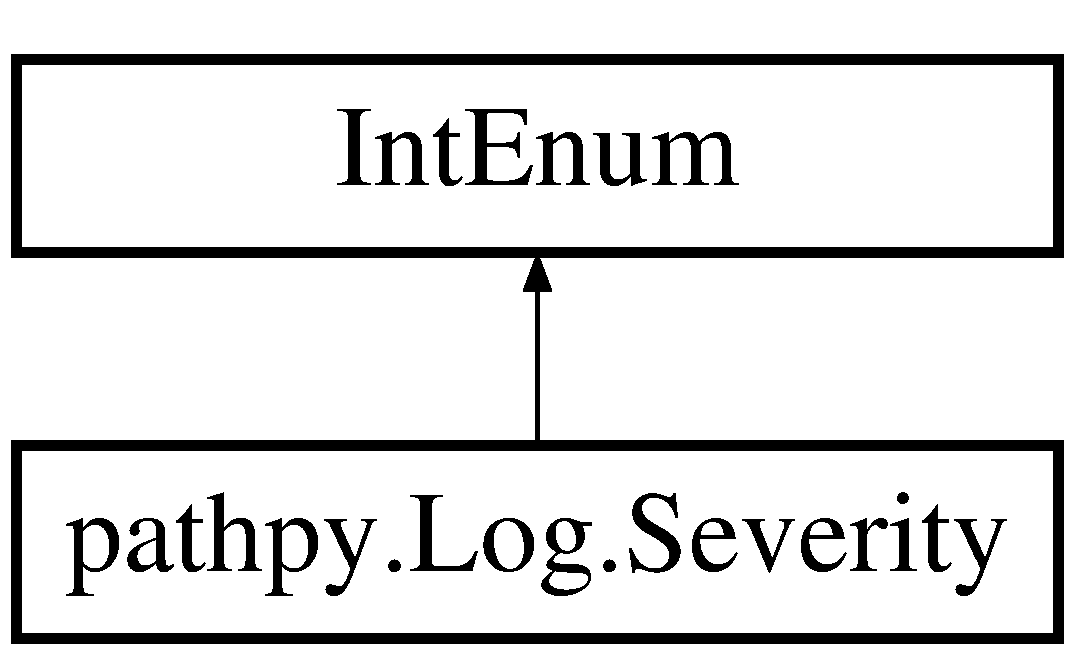
\includegraphics[height=2.000000cm]{classpathpy_1_1Log_1_1Severity}
\end{center}
\end{figure}
\subsection*{Static Public Attributes}
\begin{DoxyCompactItemize}
\item 
\hypertarget{classpathpy_1_1Log_1_1Severity_aa2e434a659bbb9f2e2c25e47fab1dc37}{int {\bfseries E\-R\-R\-O\-R} = 4}\label{classpathpy_1_1Log_1_1Severity_aa2e434a659bbb9f2e2c25e47fab1dc37}

\item 
\hypertarget{classpathpy_1_1Log_1_1Severity_ae4a13b6d9d1d2485bceb5843df6e3f40}{int {\bfseries W\-A\-R\-N\-I\-N\-G} = 3}\label{classpathpy_1_1Log_1_1Severity_ae4a13b6d9d1d2485bceb5843df6e3f40}

\item 
\hypertarget{classpathpy_1_1Log_1_1Severity_a12fb98e4cc0d9e68114e29e8f6758c22}{int {\bfseries I\-N\-F\-O} = 2}\label{classpathpy_1_1Log_1_1Severity_a12fb98e4cc0d9e68114e29e8f6758c22}

\item 
\hypertarget{classpathpy_1_1Log_1_1Severity_a0c184f8e48c1f5cb7f795d00c9205ed5}{int {\bfseries T\-I\-M\-I\-N\-G} = 1}\label{classpathpy_1_1Log_1_1Severity_a0c184f8e48c1f5cb7f795d00c9205ed5}

\item 
\hypertarget{classpathpy_1_1Log_1_1Severity_ad6d71133083c6972a8400a1e4b355381}{int {\bfseries D\-E\-B\-U\-G} = 0}\label{classpathpy_1_1Log_1_1Severity_ad6d71133083c6972a8400a1e4b355381}

\end{DoxyCompactItemize}


\subsection{Detailed Description}
\begin{DoxyVerb}An enumeration that can be used to indicate 
    the severity of log messages, and which can be 
    used tpo filter messages based on severities.
\end{DoxyVerb}
 

The documentation for this class was generated from the following file\-:\begin{DoxyCompactItemize}
\item 
/mnt/c/\-Users/ingos/\-Desktop/pathpy/pathpy/Log.\-py\end{DoxyCompactItemize}

\hypertarget{classpathpy_1_1TemporalNetwork_1_1TemporalNetwork}{\section{pathpy.\-Temporal\-Network.\-Temporal\-Network Class Reference}
\label{classpathpy_1_1TemporalNetwork_1_1TemporalNetwork}\index{pathpy.\-Temporal\-Network.\-Temporal\-Network@{pathpy.\-Temporal\-Network.\-Temporal\-Network}}
}
\subsection*{Public Member Functions}
\begin{DoxyCompactItemize}
\item 
def \hyperlink{classpathpy_1_1TemporalNetwork_1_1TemporalNetwork_a778b3b6f649c7057ac1f3f7dc3e43aff}{\-\_\-\-\_\-init\-\_\-\-\_\-}
\item 
def \hyperlink{classpathpy_1_1TemporalNetwork_1_1TemporalNetwork_a54bf4b554d7ca2a45a49cc76a0080cea}{read\-File}
\item 
def \hyperlink{classpathpy_1_1TemporalNetwork_1_1TemporalNetwork_aa1b765e6f119b214d78ba16de3b36cf4}{filter\-Edges}
\item 
def \hyperlink{classpathpy_1_1TemporalNetwork_1_1TemporalNetwork_aac7da90422a66a8123776b3d698b4615}{add\-Edge}
\item 
def \hyperlink{classpathpy_1_1TemporalNetwork_1_1TemporalNetwork_a727ebc2cc2eb2ad8c1ee23cdd5a25b6e}{vcount}
\item 
def \hyperlink{classpathpy_1_1TemporalNetwork_1_1TemporalNetwork_a040f4101e98fb4507709976c2ef7452b}{ecount}
\item 
def \hyperlink{classpathpy_1_1TemporalNetwork_1_1TemporalNetwork_a0ac006ac7818ef042fde95ea90deee80}{get\-Observation\-Length}
\item 
def \hyperlink{classpathpy_1_1TemporalNetwork_1_1TemporalNetwork_a3e43ba8b22586d6f55b2ab28a65bf35b}{get\-Inter\-Event\-Times}
\item 
def \hyperlink{classpathpy_1_1TemporalNetwork_1_1TemporalNetwork_a7a385a1b17104011975aa9c0c3f2912a}{get\-Inter\-Path\-Times}
\item 
def \hyperlink{classpathpy_1_1TemporalNetwork_1_1TemporalNetwork_a39d2b3a872f2a19554ee505393a6f708}{summary}
\item 
def \hyperlink{classpathpy_1_1TemporalNetwork_1_1TemporalNetwork_a0deb7b84090e2667840606ab0eeae509}{\-\_\-\-\_\-str\-\_\-\-\_\-}
\item 
def \hyperlink{classpathpy_1_1TemporalNetwork_1_1TemporalNetwork_a50ea38c4325e1035966c4d2173599a1d}{Shuffle\-Edges}
\item 
def \hyperlink{classpathpy_1_1TemporalNetwork_1_1TemporalNetwork_a948503bbe0104c9678778cdecfe8ceb7}{Get\-Temporal\-Betweenness}
\item 
def \hyperlink{classpathpy_1_1TemporalNetwork_1_1TemporalNetwork_aa6a91612301e802d287f1fb58fe31961}{Get\-Temporal\-Betweenness\-Instantaneous}
\item 
def \hyperlink{classpathpy_1_1TemporalNetwork_1_1TemporalNetwork_a9dd08ea1ab218cb69b2fdd56cbcab61f}{Get\-Temporal\-Closeness}
\item 
def \hyperlink{classpathpy_1_1TemporalNetwork_1_1TemporalNetwork_ac73ea9fa5c13c1df5ac101d45473243d}{Get\-Temporal\-Closeness\-Instantaneous}
\end{DoxyCompactItemize}
\subsection*{Public Attributes}
\begin{DoxyCompactItemize}
\item 
\hypertarget{classpathpy_1_1TemporalNetwork_1_1TemporalNetwork_a2ed001aa13e863e9ff6ab9ffc9ab998d}{{\bfseries tedges}}\label{classpathpy_1_1TemporalNetwork_1_1TemporalNetwork_a2ed001aa13e863e9ff6ab9ffc9ab998d}

\item 
\hypertarget{classpathpy_1_1TemporalNetwork_1_1TemporalNetwork_a86e49baf6e63c58a3f993e2768097001}{{\bfseries nodes}}\label{classpathpy_1_1TemporalNetwork_1_1TemporalNetwork_a86e49baf6e63c58a3f993e2768097001}

\item 
\hypertarget{classpathpy_1_1TemporalNetwork_1_1TemporalNetwork_a1f61dbedd4a4edde5176fec56fc1f0b3}{{\bfseries time}}\label{classpathpy_1_1TemporalNetwork_1_1TemporalNetwork_a1f61dbedd4a4edde5176fec56fc1f0b3}

\item 
\hypertarget{classpathpy_1_1TemporalNetwork_1_1TemporalNetwork_ae82b4df377620a626771cdcdcbb43b42}{{\bfseries targets}}\label{classpathpy_1_1TemporalNetwork_1_1TemporalNetwork_ae82b4df377620a626771cdcdcbb43b42}

\item 
\hypertarget{classpathpy_1_1TemporalNetwork_1_1TemporalNetwork_a0716456e27f19af5522af30e071df0ff}{{\bfseries sources}}\label{classpathpy_1_1TemporalNetwork_1_1TemporalNetwork_a0716456e27f19af5522af30e071df0ff}

\item 
\hypertarget{classpathpy_1_1TemporalNetwork_1_1TemporalNetwork_ae9ea417aa751edb7e58bc1c23602b9b8}{{\bfseries activities}}\label{classpathpy_1_1TemporalNetwork_1_1TemporalNetwork_ae9ea417aa751edb7e58bc1c23602b9b8}

\item 
\hypertarget{classpathpy_1_1TemporalNetwork_1_1TemporalNetwork_a65a5f24cb5e6cf06960f8c93c6c8aa84}{{\bfseries activities\-\_\-sets}}\label{classpathpy_1_1TemporalNetwork_1_1TemporalNetwork_a65a5f24cb5e6cf06960f8c93c6c8aa84}

\item 
\hypertarget{classpathpy_1_1TemporalNetwork_1_1TemporalNetwork_a051e7d352da3d194387762134bd70992}{{\bfseries ordered\-\_\-times}}\label{classpathpy_1_1TemporalNetwork_1_1TemporalNetwork_a051e7d352da3d194387762134bd70992}

\end{DoxyCompactItemize}


\subsection{Detailed Description}
\begin{DoxyVerb}This class represents a sequence of time-stamped edges.
   Instances of this class can be used to generate path statistics 
   based on the time-respecting paths resulting from a given maximum
   time difference between consecutive time-stamped edges.
\end{DoxyVerb}
 

\subsection{Constructor \& Destructor Documentation}
\hypertarget{classpathpy_1_1TemporalNetwork_1_1TemporalNetwork_a778b3b6f649c7057ac1f3f7dc3e43aff}{\index{pathpy\-::\-Temporal\-Network\-::\-Temporal\-Network@{pathpy\-::\-Temporal\-Network\-::\-Temporal\-Network}!\-\_\-\-\_\-init\-\_\-\-\_\-@{\-\_\-\-\_\-init\-\_\-\-\_\-}}
\index{\-\_\-\-\_\-init\-\_\-\-\_\-@{\-\_\-\-\_\-init\-\_\-\-\_\-}!pathpy::TemporalNetwork::TemporalNetwork@{pathpy\-::\-Temporal\-Network\-::\-Temporal\-Network}}
\subsubsection[{\-\_\-\-\_\-init\-\_\-\-\_\-}]{\setlength{\rightskip}{0pt plus 5cm}def pathpy.\-Temporal\-Network.\-Temporal\-Network.\-\_\-\-\_\-init\-\_\-\-\_\- (
\begin{DoxyParamCaption}
\item[{}]{self, }
\item[{}]{tedges = {\ttfamily None}}
\end{DoxyParamCaption}
)}}\label{classpathpy_1_1TemporalNetwork_1_1TemporalNetwork_a778b3b6f649c7057ac1f3f7dc3e43aff}
\begin{DoxyVerb}Constructor generating a temporal network instance

@param tedges: an optional list of (possibly unordered time-stamped) links 
    from which to construct a temporal network instance        
\end{DoxyVerb}
 

\subsection{Member Function Documentation}
\hypertarget{classpathpy_1_1TemporalNetwork_1_1TemporalNetwork_a0deb7b84090e2667840606ab0eeae509}{\index{pathpy\-::\-Temporal\-Network\-::\-Temporal\-Network@{pathpy\-::\-Temporal\-Network\-::\-Temporal\-Network}!\-\_\-\-\_\-str\-\_\-\-\_\-@{\-\_\-\-\_\-str\-\_\-\-\_\-}}
\index{\-\_\-\-\_\-str\-\_\-\-\_\-@{\-\_\-\-\_\-str\-\_\-\-\_\-}!pathpy::TemporalNetwork::TemporalNetwork@{pathpy\-::\-Temporal\-Network\-::\-Temporal\-Network}}
\subsubsection[{\-\_\-\-\_\-str\-\_\-\-\_\-}]{\setlength{\rightskip}{0pt plus 5cm}def pathpy.\-Temporal\-Network.\-Temporal\-Network.\-\_\-\-\_\-str\-\_\-\-\_\- (
\begin{DoxyParamCaption}
\item[{}]{self}
\end{DoxyParamCaption}
)}}\label{classpathpy_1_1TemporalNetwork_1_1TemporalNetwork_a0deb7b84090e2667840606ab0eeae509}
\begin{DoxyVerb}Returns the default string representation of 
this temporal network instance
\end{DoxyVerb}
 \hypertarget{classpathpy_1_1TemporalNetwork_1_1TemporalNetwork_aac7da90422a66a8123776b3d698b4615}{\index{pathpy\-::\-Temporal\-Network\-::\-Temporal\-Network@{pathpy\-::\-Temporal\-Network\-::\-Temporal\-Network}!add\-Edge@{add\-Edge}}
\index{add\-Edge@{add\-Edge}!pathpy::TemporalNetwork::TemporalNetwork@{pathpy\-::\-Temporal\-Network\-::\-Temporal\-Network}}
\subsubsection[{add\-Edge}]{\setlength{\rightskip}{0pt plus 5cm}def pathpy.\-Temporal\-Network.\-Temporal\-Network.\-add\-Edge (
\begin{DoxyParamCaption}
\item[{}]{self, }
\item[{}]{source, }
\item[{}]{target, }
\item[{}]{ts}
\end{DoxyParamCaption}
)}}\label{classpathpy_1_1TemporalNetwork_1_1TemporalNetwork_aac7da90422a66a8123776b3d698b4615}
\begin{DoxyVerb}Adds a directed time-stamped edge (source,target;time) to the temporal network. To add an undirected 
    time-stamped link (u,v;t) at time t, please call addEdge(u,v;t) and addEdge(v,u;t).

@param source: naem of the source node of a directed, time-stamped link
@param target: name of the target node of a directed, time-stamped link
@param ts: (integer) time-stamp of the time-stamped link
\end{DoxyVerb}
 \hypertarget{classpathpy_1_1TemporalNetwork_1_1TemporalNetwork_a040f4101e98fb4507709976c2ef7452b}{\index{pathpy\-::\-Temporal\-Network\-::\-Temporal\-Network@{pathpy\-::\-Temporal\-Network\-::\-Temporal\-Network}!ecount@{ecount}}
\index{ecount@{ecount}!pathpy::TemporalNetwork::TemporalNetwork@{pathpy\-::\-Temporal\-Network\-::\-Temporal\-Network}}
\subsubsection[{ecount}]{\setlength{\rightskip}{0pt plus 5cm}def pathpy.\-Temporal\-Network.\-Temporal\-Network.\-ecount (
\begin{DoxyParamCaption}
\item[{}]{self}
\end{DoxyParamCaption}
)}}\label{classpathpy_1_1TemporalNetwork_1_1TemporalNetwork_a040f4101e98fb4507709976c2ef7452b}
\begin{DoxyVerb}Returns the number of time-stamped edges (u,v;t)
\end{DoxyVerb}
 \hypertarget{classpathpy_1_1TemporalNetwork_1_1TemporalNetwork_aa1b765e6f119b214d78ba16de3b36cf4}{\index{pathpy\-::\-Temporal\-Network\-::\-Temporal\-Network@{pathpy\-::\-Temporal\-Network\-::\-Temporal\-Network}!filter\-Edges@{filter\-Edges}}
\index{filter\-Edges@{filter\-Edges}!pathpy::TemporalNetwork::TemporalNetwork@{pathpy\-::\-Temporal\-Network\-::\-Temporal\-Network}}
\subsubsection[{filter\-Edges}]{\setlength{\rightskip}{0pt plus 5cm}def pathpy.\-Temporal\-Network.\-Temporal\-Network.\-filter\-Edges (
\begin{DoxyParamCaption}
\item[{}]{self, }
\item[{}]{edge\-\_\-filter}
\end{DoxyParamCaption}
)}}\label{classpathpy_1_1TemporalNetwork_1_1TemporalNetwork_aa1b765e6f119b214d78ba16de3b36cf4}
\begin{DoxyVerb}Filter time-stamped edges according to a given filter expression. 

@param edge_filter: an arbitrary filter function of the form filter_func(v, w, time) that 
    returns True for time-stamped edges that shall pass the filter, and False for all edges that 
    shall be filtered out.
\end{DoxyVerb}
 \hypertarget{classpathpy_1_1TemporalNetwork_1_1TemporalNetwork_a3e43ba8b22586d6f55b2ab28a65bf35b}{\index{pathpy\-::\-Temporal\-Network\-::\-Temporal\-Network@{pathpy\-::\-Temporal\-Network\-::\-Temporal\-Network}!get\-Inter\-Event\-Times@{get\-Inter\-Event\-Times}}
\index{get\-Inter\-Event\-Times@{get\-Inter\-Event\-Times}!pathpy::TemporalNetwork::TemporalNetwork@{pathpy\-::\-Temporal\-Network\-::\-Temporal\-Network}}
\subsubsection[{get\-Inter\-Event\-Times}]{\setlength{\rightskip}{0pt plus 5cm}def pathpy.\-Temporal\-Network.\-Temporal\-Network.\-get\-Inter\-Event\-Times (
\begin{DoxyParamCaption}
\item[{}]{self}
\end{DoxyParamCaption}
)}}\label{classpathpy_1_1TemporalNetwork_1_1TemporalNetwork_a3e43ba8b22586d6f55b2ab28a65bf35b}
\begin{DoxyVerb}Returns a numpy array containing all time differences between any 
two consecutive time-stamped links (involving any node)
\end{DoxyVerb}
 \hypertarget{classpathpy_1_1TemporalNetwork_1_1TemporalNetwork_a7a385a1b17104011975aa9c0c3f2912a}{\index{pathpy\-::\-Temporal\-Network\-::\-Temporal\-Network@{pathpy\-::\-Temporal\-Network\-::\-Temporal\-Network}!get\-Inter\-Path\-Times@{get\-Inter\-Path\-Times}}
\index{get\-Inter\-Path\-Times@{get\-Inter\-Path\-Times}!pathpy::TemporalNetwork::TemporalNetwork@{pathpy\-::\-Temporal\-Network\-::\-Temporal\-Network}}
\subsubsection[{get\-Inter\-Path\-Times}]{\setlength{\rightskip}{0pt plus 5cm}def pathpy.\-Temporal\-Network.\-Temporal\-Network.\-get\-Inter\-Path\-Times (
\begin{DoxyParamCaption}
\item[{}]{self}
\end{DoxyParamCaption}
)}}\label{classpathpy_1_1TemporalNetwork_1_1TemporalNetwork_a7a385a1b17104011975aa9c0c3f2912a}
\begin{DoxyVerb}Returns a dictionary which, for each node v, contains all time differences 
between any time-stamped link (*,v;t) and the next link (v,*;t') (t'>t)
in the temporal network
\end{DoxyVerb}
 \hypertarget{classpathpy_1_1TemporalNetwork_1_1TemporalNetwork_a0ac006ac7818ef042fde95ea90deee80}{\index{pathpy\-::\-Temporal\-Network\-::\-Temporal\-Network@{pathpy\-::\-Temporal\-Network\-::\-Temporal\-Network}!get\-Observation\-Length@{get\-Observation\-Length}}
\index{get\-Observation\-Length@{get\-Observation\-Length}!pathpy::TemporalNetwork::TemporalNetwork@{pathpy\-::\-Temporal\-Network\-::\-Temporal\-Network}}
\subsubsection[{get\-Observation\-Length}]{\setlength{\rightskip}{0pt plus 5cm}def pathpy.\-Temporal\-Network.\-Temporal\-Network.\-get\-Observation\-Length (
\begin{DoxyParamCaption}
\item[{}]{self}
\end{DoxyParamCaption}
)}}\label{classpathpy_1_1TemporalNetwork_1_1TemporalNetwork_a0ac006ac7818ef042fde95ea90deee80}
\begin{DoxyVerb}Returns the length of the observation time.
\end{DoxyVerb}
 \hypertarget{classpathpy_1_1TemporalNetwork_1_1TemporalNetwork_a948503bbe0104c9678778cdecfe8ceb7}{\index{pathpy\-::\-Temporal\-Network\-::\-Temporal\-Network@{pathpy\-::\-Temporal\-Network\-::\-Temporal\-Network}!Get\-Temporal\-Betweenness@{Get\-Temporal\-Betweenness}}
\index{Get\-Temporal\-Betweenness@{Get\-Temporal\-Betweenness}!pathpy::TemporalNetwork::TemporalNetwork@{pathpy\-::\-Temporal\-Network\-::\-Temporal\-Network}}
\subsubsection[{Get\-Temporal\-Betweenness}]{\setlength{\rightskip}{0pt plus 5cm}def pathpy.\-Temporal\-Network.\-Temporal\-Network.\-Get\-Temporal\-Betweenness (
\begin{DoxyParamCaption}
\item[{}]{t, }
\item[{}]{delta = {\ttfamily 1}, }
\item[{}]{normalized = {\ttfamily False}}
\end{DoxyParamCaption}
)}}\label{classpathpy_1_1TemporalNetwork_1_1TemporalNetwork_a948503bbe0104c9678778cdecfe8ceb7}
\begin{DoxyVerb}Calculates the temporal betweenness centralities of all nodes based on the shortest 
time-respecting paths with a maximum waiting time of delta. This function returns a 
numpy array of temporal betweenness centrality values of nodes.
    
@param t: the temporal network for which temporal closeness centralities will be computed    
@param delta: the maximum time difference used in the time-respecting path definition (default 1).
    Note that this parameter is independent from the delta used internally for the extraction 
    of two-paths by the class TemporalNetwork
@param normalized: whether or not to normalize centralities by dividing each value by the total 
    number of shortest time-respecting paths.
\end{DoxyVerb}
 \hypertarget{classpathpy_1_1TemporalNetwork_1_1TemporalNetwork_aa6a91612301e802d287f1fb58fe31961}{\index{pathpy\-::\-Temporal\-Network\-::\-Temporal\-Network@{pathpy\-::\-Temporal\-Network\-::\-Temporal\-Network}!Get\-Temporal\-Betweenness\-Instantaneous@{Get\-Temporal\-Betweenness\-Instantaneous}}
\index{Get\-Temporal\-Betweenness\-Instantaneous@{Get\-Temporal\-Betweenness\-Instantaneous}!pathpy::TemporalNetwork::TemporalNetwork@{pathpy\-::\-Temporal\-Network\-::\-Temporal\-Network}}
\subsubsection[{Get\-Temporal\-Betweenness\-Instantaneous}]{\setlength{\rightskip}{0pt plus 5cm}def pathpy.\-Temporal\-Network.\-Temporal\-Network.\-Get\-Temporal\-Betweenness\-Instantaneous (
\begin{DoxyParamCaption}
\item[{}]{t, }
\item[{}]{start\-\_\-t = {\ttfamily 0}, }
\item[{}]{delta = {\ttfamily 1}, }
\item[{}]{normalized = {\ttfamily False}}
\end{DoxyParamCaption}
)}}\label{classpathpy_1_1TemporalNetwork_1_1TemporalNetwork_aa6a91612301e802d287f1fb58fe31961}
\begin{DoxyVerb}Calculates the temporal betweennness values of 
all nodes fir a given start time start_t in an empirical temporal network t.
This function returns a numpy array of (temporal) betweenness centrality values. 
The ordering of these values corresponds to the ordering of nodes in the vertex 
sequence of the igraph first order time-aggregated network. A mapping between node names
and array indices can be found in Utilities.firstOrderNameMap().
    
@param t: the temporal network for which temporal betweenness centralities will be computed
@param start_t: the start time for which to consider time-respecting paths (default 0). This is 
    important, since any unambigious definition of a shortest time-respecting path between
    two nodes must include the time range to be considered (c.f. Holme and Saramäki, Phys. Rep., 2012)
@param delta: the maximum waiting time used in the time-respecting path definition (default 1)
    Note that this parameter is independent from the delta used internally for the extraction of two-paths
    by the class TemporalNetwork
@param normalized: whether or not to normalize the temporal betweenness centrality values by
    dividing by the number of all shortest time-respecting paths in the temporal network.
\end{DoxyVerb}
 \hypertarget{classpathpy_1_1TemporalNetwork_1_1TemporalNetwork_a9dd08ea1ab218cb69b2fdd56cbcab61f}{\index{pathpy\-::\-Temporal\-Network\-::\-Temporal\-Network@{pathpy\-::\-Temporal\-Network\-::\-Temporal\-Network}!Get\-Temporal\-Closeness@{Get\-Temporal\-Closeness}}
\index{Get\-Temporal\-Closeness@{Get\-Temporal\-Closeness}!pathpy::TemporalNetwork::TemporalNetwork@{pathpy\-::\-Temporal\-Network\-::\-Temporal\-Network}}
\subsubsection[{Get\-Temporal\-Closeness}]{\setlength{\rightskip}{0pt plus 5cm}def pathpy.\-Temporal\-Network.\-Temporal\-Network.\-Get\-Temporal\-Closeness (
\begin{DoxyParamCaption}
\item[{}]{t, }
\item[{}]{delta = {\ttfamily 1}}
\end{DoxyParamCaption}
)}}\label{classpathpy_1_1TemporalNetwork_1_1TemporalNetwork_a9dd08ea1ab218cb69b2fdd56cbcab61f}
\begin{DoxyVerb}Calculates the temporal closeness centralities of all nodes based on the minimal 
shortest time-respecting paths with a maximum time difference of delta. This function 
returns a numpy array of average (temporal) closeness centrality values of nodes.
    
@param t: the temporal network for which temporal closeness centralities will be computed   
@param delta: the maximum waiting time used in the time-respecting path definition (default 1)            
\end{DoxyVerb}
 \hypertarget{classpathpy_1_1TemporalNetwork_1_1TemporalNetwork_ac73ea9fa5c13c1df5ac101d45473243d}{\index{pathpy\-::\-Temporal\-Network\-::\-Temporal\-Network@{pathpy\-::\-Temporal\-Network\-::\-Temporal\-Network}!Get\-Temporal\-Closeness\-Instantaneous@{Get\-Temporal\-Closeness\-Instantaneous}}
\index{Get\-Temporal\-Closeness\-Instantaneous@{Get\-Temporal\-Closeness\-Instantaneous}!pathpy::TemporalNetwork::TemporalNetwork@{pathpy\-::\-Temporal\-Network\-::\-Temporal\-Network}}
\subsubsection[{Get\-Temporal\-Closeness\-Instantaneous}]{\setlength{\rightskip}{0pt plus 5cm}def pathpy.\-Temporal\-Network.\-Temporal\-Network.\-Get\-Temporal\-Closeness\-Instantaneous (
\begin{DoxyParamCaption}
\item[{}]{t, }
\item[{}]{start\-\_\-t = {\ttfamily 0}, }
\item[{}]{delta = {\ttfamily 1}}
\end{DoxyParamCaption}
)}}\label{classpathpy_1_1TemporalNetwork_1_1TemporalNetwork_ac73ea9fa5c13c1df5ac101d45473243d}
\begin{DoxyVerb}Calculates the temporal closeness values of all nodes for a given start time start_t.
This function returns a numpy array of (temporal) closeness centrality values.        
    
@param t: the temporal network for which temporal closeness centralities will be computed
@param start_t: the start time for which to consider time-respecting paths (default 0). This is 
    important, since any unambigious definition of a shortest time-respecting path between
    two nodes must include the time range to be considered (c.f. Holme and Saramäki, Phys. Rep., 2012)
@param delta: the maximum time difference time used in the time-respecting path definition (default 1)
    Note that this parameter is independent from the delta used internally for the extraction of two-paths
    by the class TemporalNetwork.
\end{DoxyVerb}
 \hypertarget{classpathpy_1_1TemporalNetwork_1_1TemporalNetwork_a54bf4b554d7ca2a45a49cc76a0080cea}{\index{pathpy\-::\-Temporal\-Network\-::\-Temporal\-Network@{pathpy\-::\-Temporal\-Network\-::\-Temporal\-Network}!read\-File@{read\-File}}
\index{read\-File@{read\-File}!pathpy::TemporalNetwork::TemporalNetwork@{pathpy\-::\-Temporal\-Network\-::\-Temporal\-Network}}
\subsubsection[{read\-File}]{\setlength{\rightskip}{0pt plus 5cm}def pathpy.\-Temporal\-Network.\-Temporal\-Network.\-read\-File (
\begin{DoxyParamCaption}
\item[{}]{filename = {\ttfamily ''}, }
\item[{}]{sep = {\ttfamily '}, }
\item[{}]{timestampformat = {\ttfamily \char`\"{}\%s\char`\"{}}, }
\item[{}]{maxlines = {\ttfamily \-\_\-sys.maxsize}}
\end{DoxyParamCaption}
)}}\label{classpathpy_1_1TemporalNetwork_1_1TemporalNetwork_a54bf4b554d7ca2a45a49cc76a0080cea}
\begin{DoxyVerb}Reads time-stamped links from a file and returns a new instance 
    of the class TemporalNetwork
\end{DoxyVerb}
 \hypertarget{classpathpy_1_1TemporalNetwork_1_1TemporalNetwork_a50ea38c4325e1035966c4d2173599a1d}{\index{pathpy\-::\-Temporal\-Network\-::\-Temporal\-Network@{pathpy\-::\-Temporal\-Network\-::\-Temporal\-Network}!Shuffle\-Edges@{Shuffle\-Edges}}
\index{Shuffle\-Edges@{Shuffle\-Edges}!pathpy::TemporalNetwork::TemporalNetwork@{pathpy\-::\-Temporal\-Network\-::\-Temporal\-Network}}
\subsubsection[{Shuffle\-Edges}]{\setlength{\rightskip}{0pt plus 5cm}def pathpy.\-Temporal\-Network.\-Temporal\-Network.\-Shuffle\-Edges (
\begin{DoxyParamCaption}
\item[{}]{self, }
\item[{}]{l = {\ttfamily 0}, }
\item[{}]{with\-\_\-replacement = {\ttfamily False}}
\end{DoxyParamCaption}
)}}\label{classpathpy_1_1TemporalNetwork_1_1TemporalNetwork_a50ea38c4325e1035966c4d2173599a1d}
\begin{DoxyVerb}Generates a shuffled version of the temporal network in which edge statistics (i.e.
the frequencies of time-stamped edges) are preserved, while all order correlations are 
destroyed. The shuffling procedure randomly reshuffles the time-stamps of links.

@param l: the length of the sequence to be generated (i.e. the number of time-stamped links.
    For the default value l=0, the length of the generated shuffled temporal network will be 
    equal to that of the original temporal network. 
\end{DoxyVerb}
 \hypertarget{classpathpy_1_1TemporalNetwork_1_1TemporalNetwork_a39d2b3a872f2a19554ee505393a6f708}{\index{pathpy\-::\-Temporal\-Network\-::\-Temporal\-Network@{pathpy\-::\-Temporal\-Network\-::\-Temporal\-Network}!summary@{summary}}
\index{summary@{summary}!pathpy::TemporalNetwork::TemporalNetwork@{pathpy\-::\-Temporal\-Network\-::\-Temporal\-Network}}
\subsubsection[{summary}]{\setlength{\rightskip}{0pt plus 5cm}def pathpy.\-Temporal\-Network.\-Temporal\-Network.\-summary (
\begin{DoxyParamCaption}
\item[{}]{self}
\end{DoxyParamCaption}
)}}\label{classpathpy_1_1TemporalNetwork_1_1TemporalNetwork_a39d2b3a872f2a19554ee505393a6f708}
\begin{DoxyVerb}Returns a string containing basic summary statistics of this temporal network
\end{DoxyVerb}
 \hypertarget{classpathpy_1_1TemporalNetwork_1_1TemporalNetwork_a727ebc2cc2eb2ad8c1ee23cdd5a25b6e}{\index{pathpy\-::\-Temporal\-Network\-::\-Temporal\-Network@{pathpy\-::\-Temporal\-Network\-::\-Temporal\-Network}!vcount@{vcount}}
\index{vcount@{vcount}!pathpy::TemporalNetwork::TemporalNetwork@{pathpy\-::\-Temporal\-Network\-::\-Temporal\-Network}}
\subsubsection[{vcount}]{\setlength{\rightskip}{0pt plus 5cm}def pathpy.\-Temporal\-Network.\-Temporal\-Network.\-vcount (
\begin{DoxyParamCaption}
\item[{}]{self}
\end{DoxyParamCaption}
)}}\label{classpathpy_1_1TemporalNetwork_1_1TemporalNetwork_a727ebc2cc2eb2ad8c1ee23cdd5a25b6e}
\begin{DoxyVerb}Returns the total number of different vertices active across the whole evolution of the 
temporal network. This number corresponds to the number of nodes in the (first-order) 
time-aggregated network.
\end{DoxyVerb}
 

The documentation for this class was generated from the following file\-:\begin{DoxyCompactItemize}
\item 
/mnt/c/\-Users/ingos/\-Desktop/pathpy/pathpy/Temporal\-Network.\-py\end{DoxyCompactItemize}

%--- End generated contents ---

% Index
\newpage
\phantomsection
\addcontentsline{toc}{chapter}{Index}
\printindex

\end{document}
